\documentclass[12pt,a4paper,titlepage]{article}
\usepackage[utf8]{inputenc}
\usepackage{amsmath}
\usepackage{amsfonts}
\usepackage{amssymb}
\usepackage{fancyhdr}
\usepackage{placeins}
\usepackage{datetime}

\pagestyle{fancy}

\renewcommand{\sectionmark}[1]{%
\markboth{#1}{}}
\fancyhf{} % delete current header and footer
\fancyhead[R]{\bfseries\leftmark}
\fancyfoot[R]{Page \thepage}
\renewcommand{\headrulewidth}{0.5pt}
\renewcommand{\footrulewidth}{0.5pt}
\addtolength{\headheight}{2.5pt} % space for the rule

\fancypagestyle{plain}{%
\fancyhead{} % get rid of headers on plain pages
\fancyfoot{} % get rid of headers on plain pages
}

\usepackage[pdftex]{graphicx}
\author{PA Nilsson}
\title{KEEP Quick Start}
\usepackage[pdftex,colorlinks]{hyperref}
\begin{document}
%\maketitle
\FloatBarrier
\section{Installing KEEP is Easy}
	\begin{enumerate}

		\item Plug in the network cable to in Internet enabled port, either directly connected to the Internet or behind a router.

		\item Connect the power supply to a mains outlet and plug it into KEEP. KEEP is designed with the intention of being placed close to your router, so the provided ethernet cable is fairly short in order not cause more cable fuss than necessary.

		\item Wait for the LED to start flashing green with heartbeat pattern. This means that KEEP is ready for initialization.

		\item During the order/delivery process for KEEP, you should have received an email with an url to active your unit. The url is in the format of

\begin{small}
https://setup.op-i.me/index.php?unit\_id=41c189de-83e1-47a2-9a6d-a1d61929b01
\end{small}

Follow that link and follow the instruction on screen to complete the setup.

\end{enumerate}
\begin{quote}
\emph{\textbf{
Note that the master password you select is not stored anywhere and can not be emailed to you if you loose it.
}}

\emph{\textbf{
KEEP is designed to keep your information secure, and all personal information is stored encrypted on KEEP. To accomplish this you will need to provide the password on each restart to unlock KEEP.}}

\emph{\textbf{ Without the password all data is encrypted on the disk and not accessible even if you remove the drive.
}}
\end{quote}

\begin{center}
	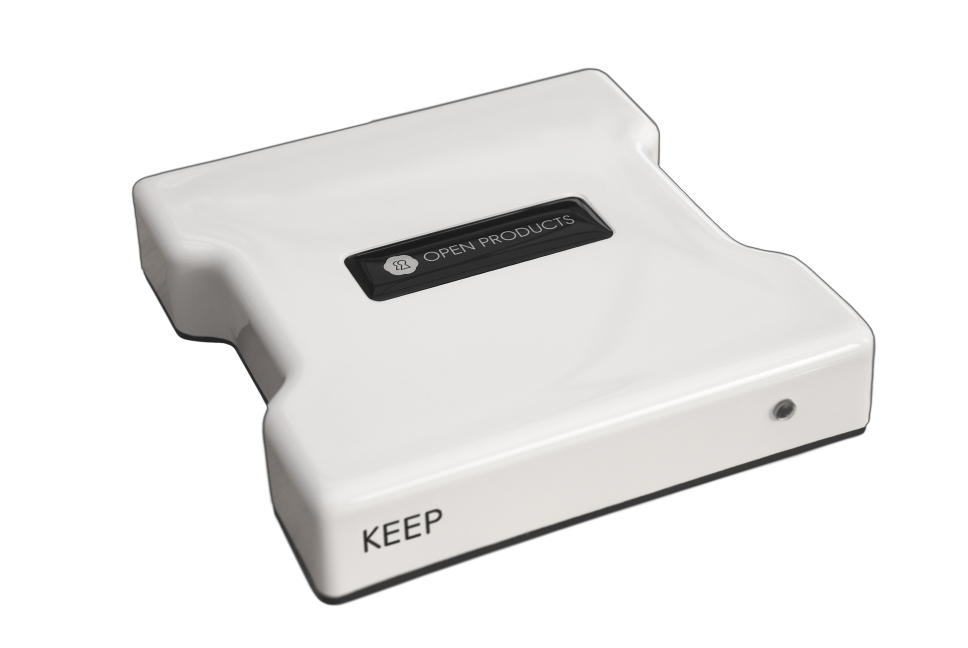
\includegraphics[width=7cm]{./img/KEEP-front}
\end{center}

\FloatBarrier
\newpage
\section{It Was Not THAT Easy\ldots}
For some reason the above process did not work, let us try to figure out why.
\begin{itemize}
\item \textbf{The page says that I can not reach KEEP.}

This is most likely caused by a firewall. KEEP tries to open and forwards ports using upnp, but not all firewall/routers are configured to accept that.

To proceed you must either:
\begin{enumerate}
\item Forward at least https traffic (port 443) to KEEP
\end{enumerate}
\emph{or}
\begin{enumerate}
\setcounter{enumi}{1}
\item Access KEEP from within your local network. In your local network you should be able to reach KEEP on https://keep
\end{enumerate}

Note that you must use \emph{https} (encrypted connection) not just http.

Hopefully you will now be prompted to enter the long activation number from your order confirmation email together and the master password.
Then follow the instructions on screen.
\end{itemize}
\FloatBarrier
\newpage
\section{Init Process – Step by Step}
\subsection{Master Password Selection}
\begin{figure}[h!]
\centering
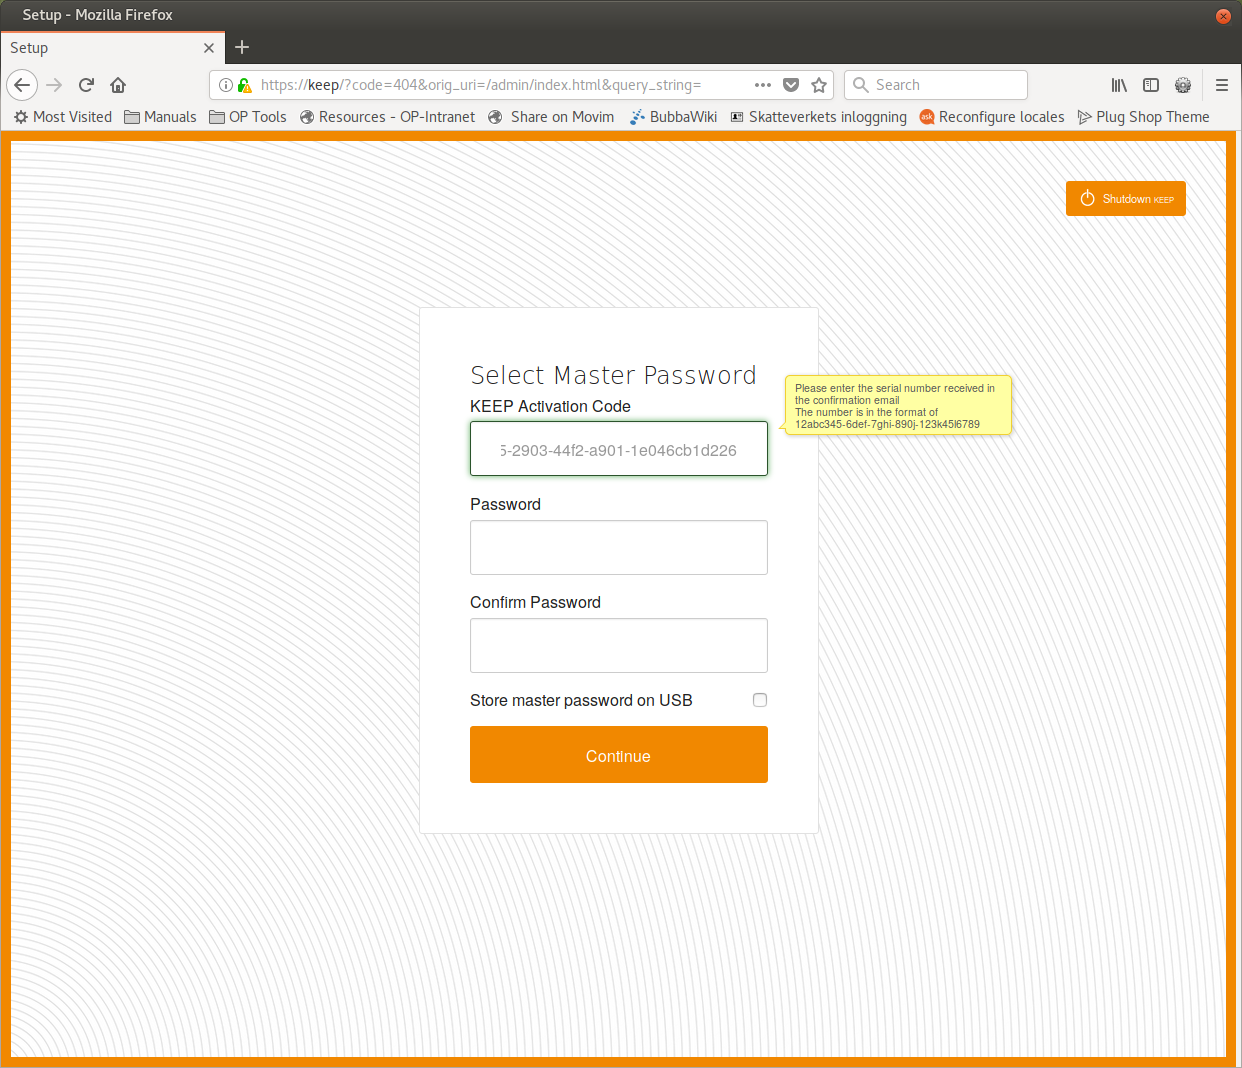
\includegraphics[width=10cm]{./img/master_pwd}
\caption{Master Password selection}
\end{figure}

The first thing that needs to be done is to choose a master password for KEEP. This password is used as a seed for the key that is used to encrypt all information on KEEP.

\begin{quote}
\emph{\textbf{The password itself is not stored anywhere and can not be recovered or sent to you by email}.\\
If you loose this password, there is no way to access your information.}
\end{quote}

So be very careful and if you are not sure you can remember it, write it down and store it somewhere safe. Although KEEP would be a perfect place to store such sensitive information, we do not encourage you to store your master password on KEEP.
That will pose some great challenges when needed to unlock KEEP....

Once the master password is chosen and entered, KEEP will encrypt the memory card using the supplied password. This takes some time, so just be patient, leave the browser open and if you have a big disk, go get a cup of coffee.

By checking the box ``Store password on USB'' the password will be stored on USB, provided that there is a USB mass storage device inserted in the USB port of KEEP. It the USB device is then present on when KEEP is booting, the master password will be read from that device and KEEP will be unlocked automatically. While this might be a very smooth setup, it also limits the data protection in case of theft since the master password will be available to unlock KEEP.

The initial setup includes encryption of the storage area as well as generating keys for authentication and takes a while, so be patient during this process.
\begin{figure}[h!]
\centering
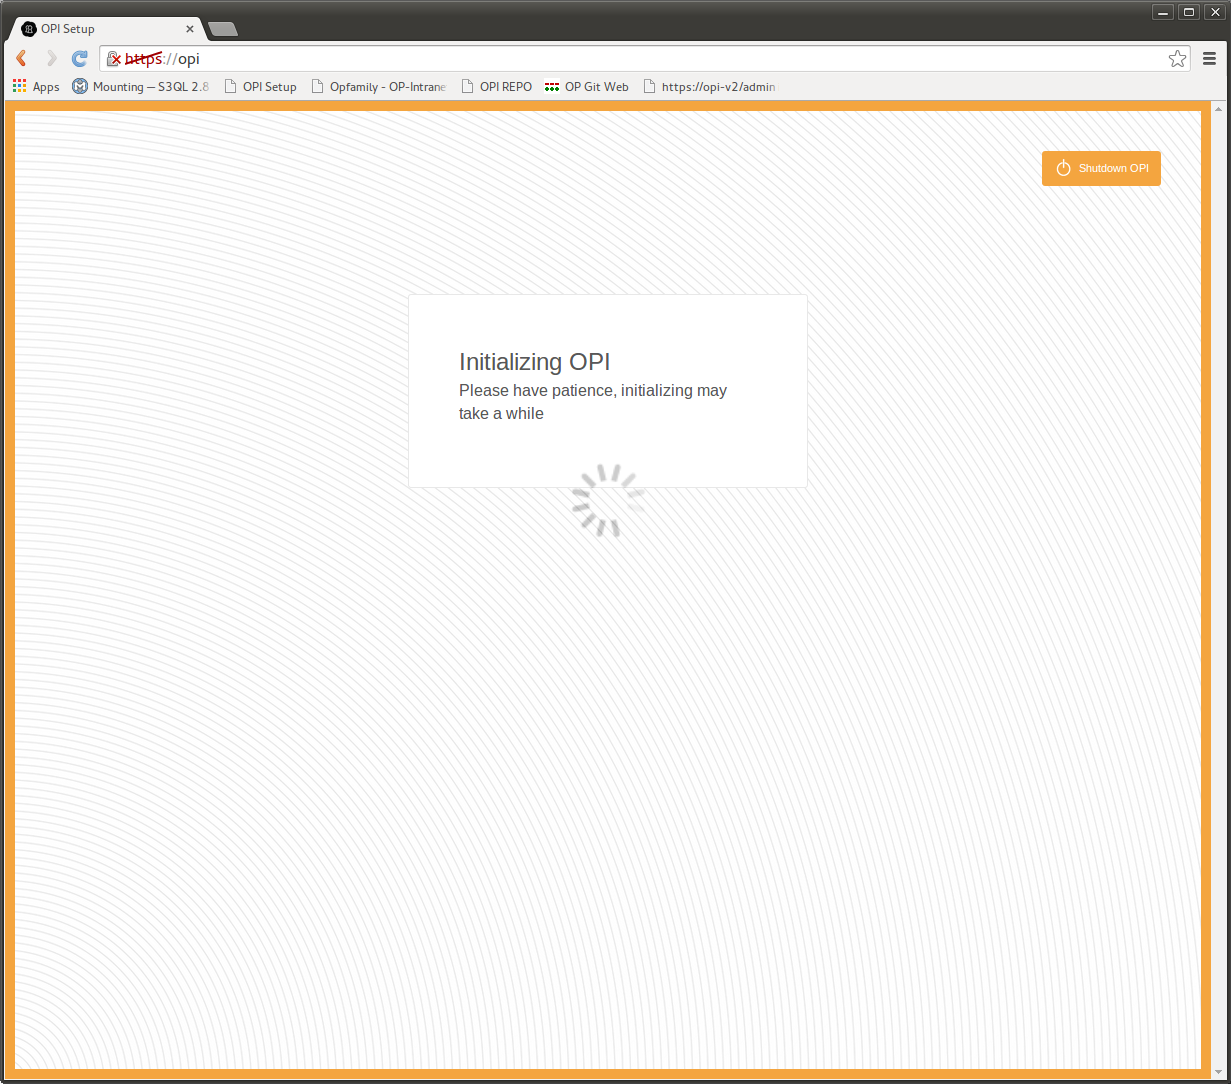
\includegraphics[width=10cm]{./img/init}
\caption{Initializing KEEP}
\end{figure}

\newpage
\subsection{Restore Data}
\begin{figure}[h!]
\centering
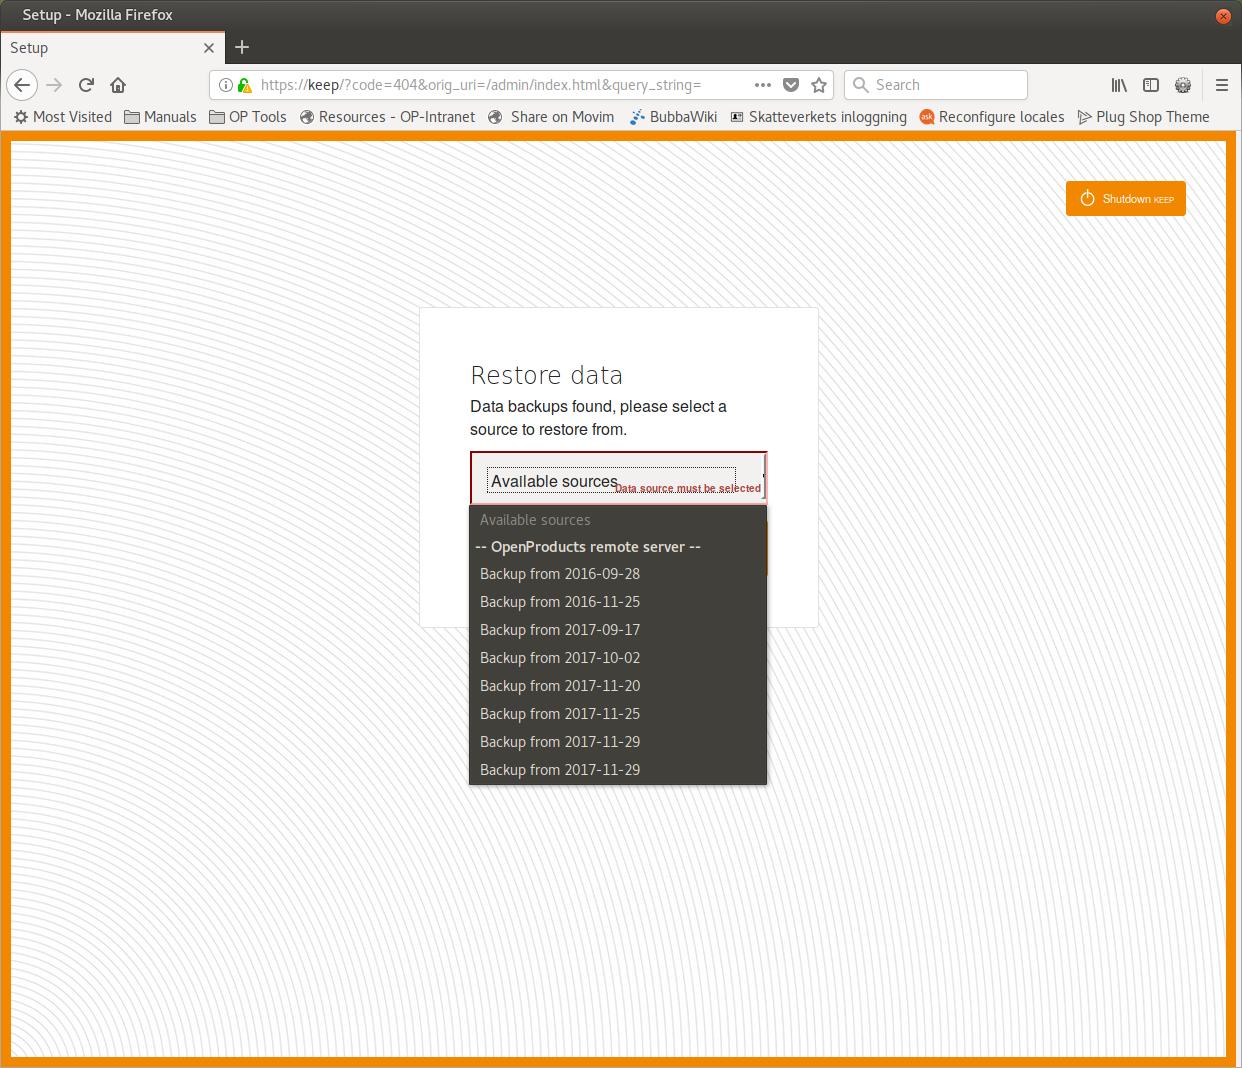
\includegraphics[width=10cm]{./img/restore}
\caption{Selecting Data Source}
\end{figure}
Only if the device can find and access any previous data backups this step will be shown. Any data sources found, either on remote on OpenProducts Servers or local on USB these will be listed in the dropdown menu. To restore data, simply choose the set that should be used to restore data from. All data will then be restored, including users and their mail, files, contacts and calendars.

Pressing "Skip Restore" will do a clean install, not restoring any data.

\newpage
\subsection{Add First User}
\begin{figure}[h!]
\centering
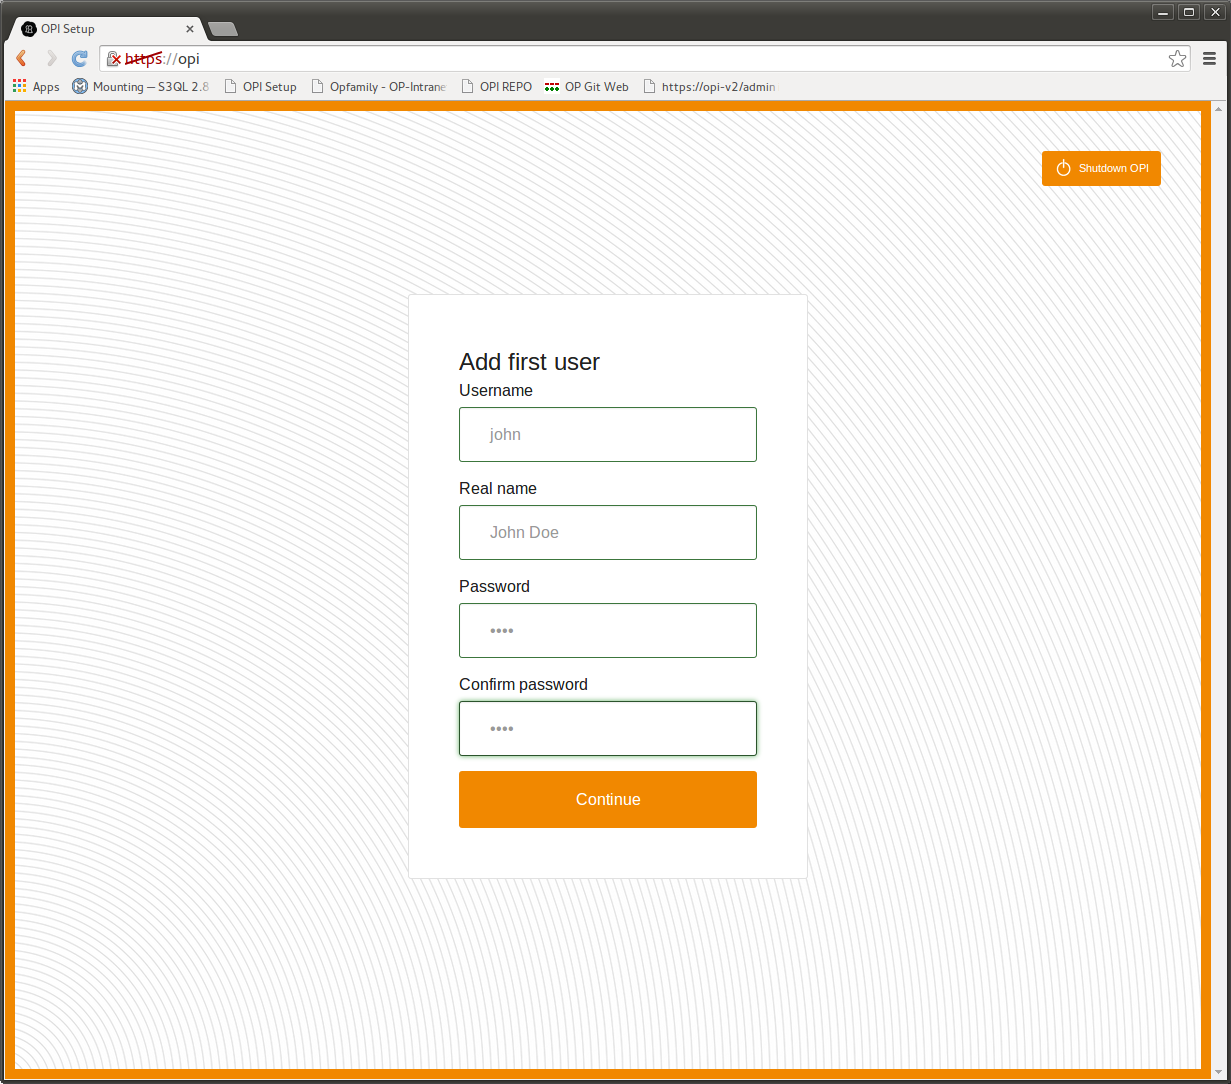
\includegraphics[width=10cm]{./img/first_user}
\caption{Adding First User}
\end{figure}
Once the master password has been set, the next step is to add the first user. Enter the users real name, also known in the system as ``Display name'', username and password. The first user entered will also be added to the ``admin'' group, given access to configure the system.

\newpage
\subsection{Select your Device Name}
\begin{figure}[h!]
\centering
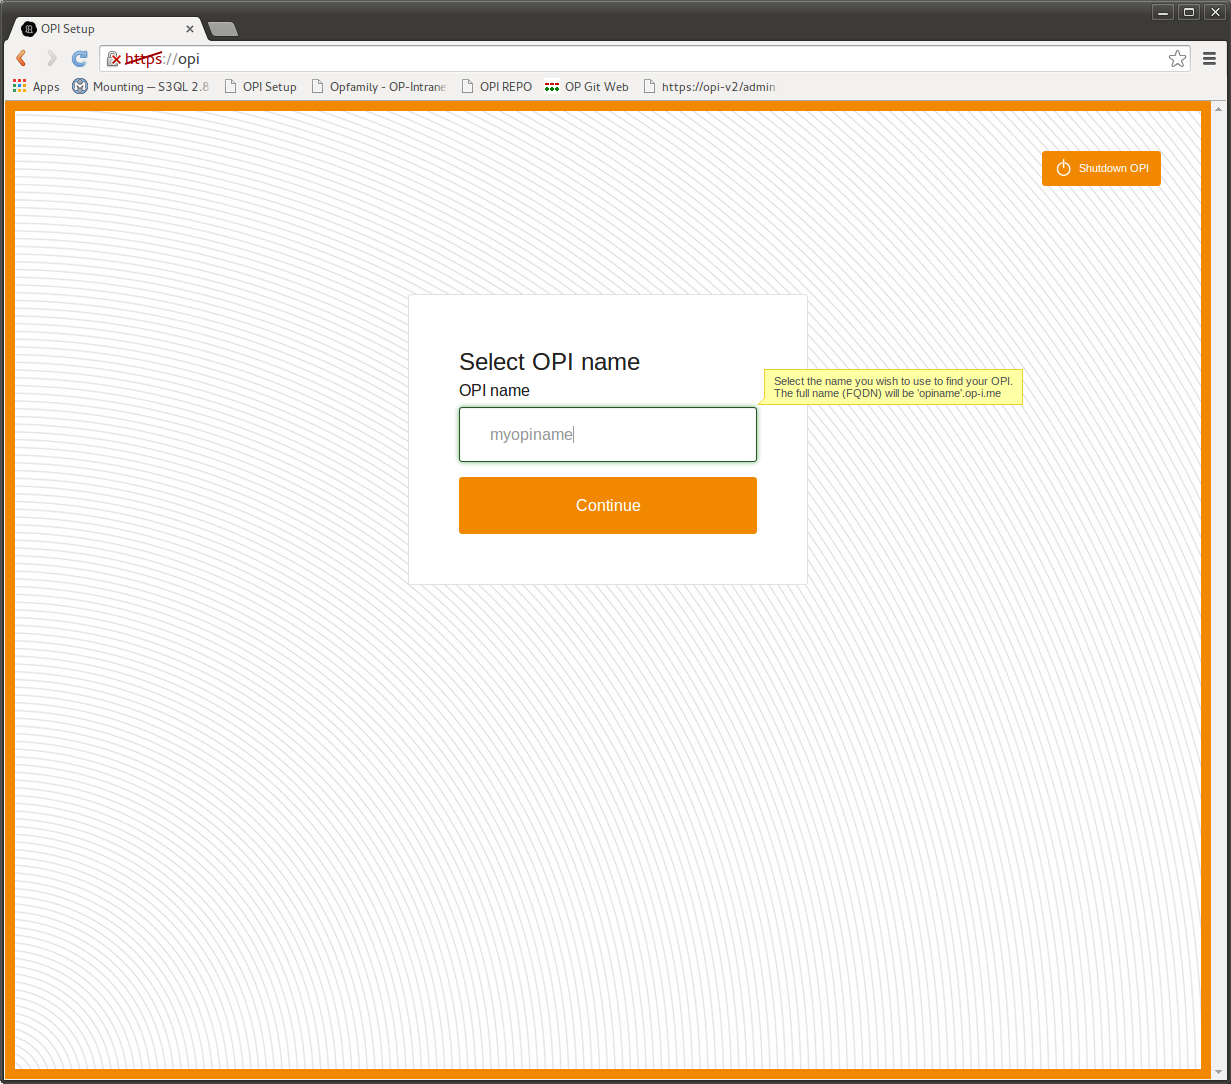
\includegraphics[width=10cm]{./img/opiname}
\caption{Selecting KEEP name}
\end{figure}
In order to find and access KEEP over the Internet a domain name needs to be associated with your unit. OpenProducts provides this service, free of charge for all OPIs and KEEPs under the domains “op-i.me” or "mykeep.net", selectable in the drop down list.

In this step you can select a name that prepends the domain name and makes it possible to find your unit. KEEP then automatically updates this name if your IP address is changed.

\newpage
\subsection{KEEP is unlocked}
All required setups is now complete and you are ready to start using your unit.
\begin{figure}[h!]
\centering
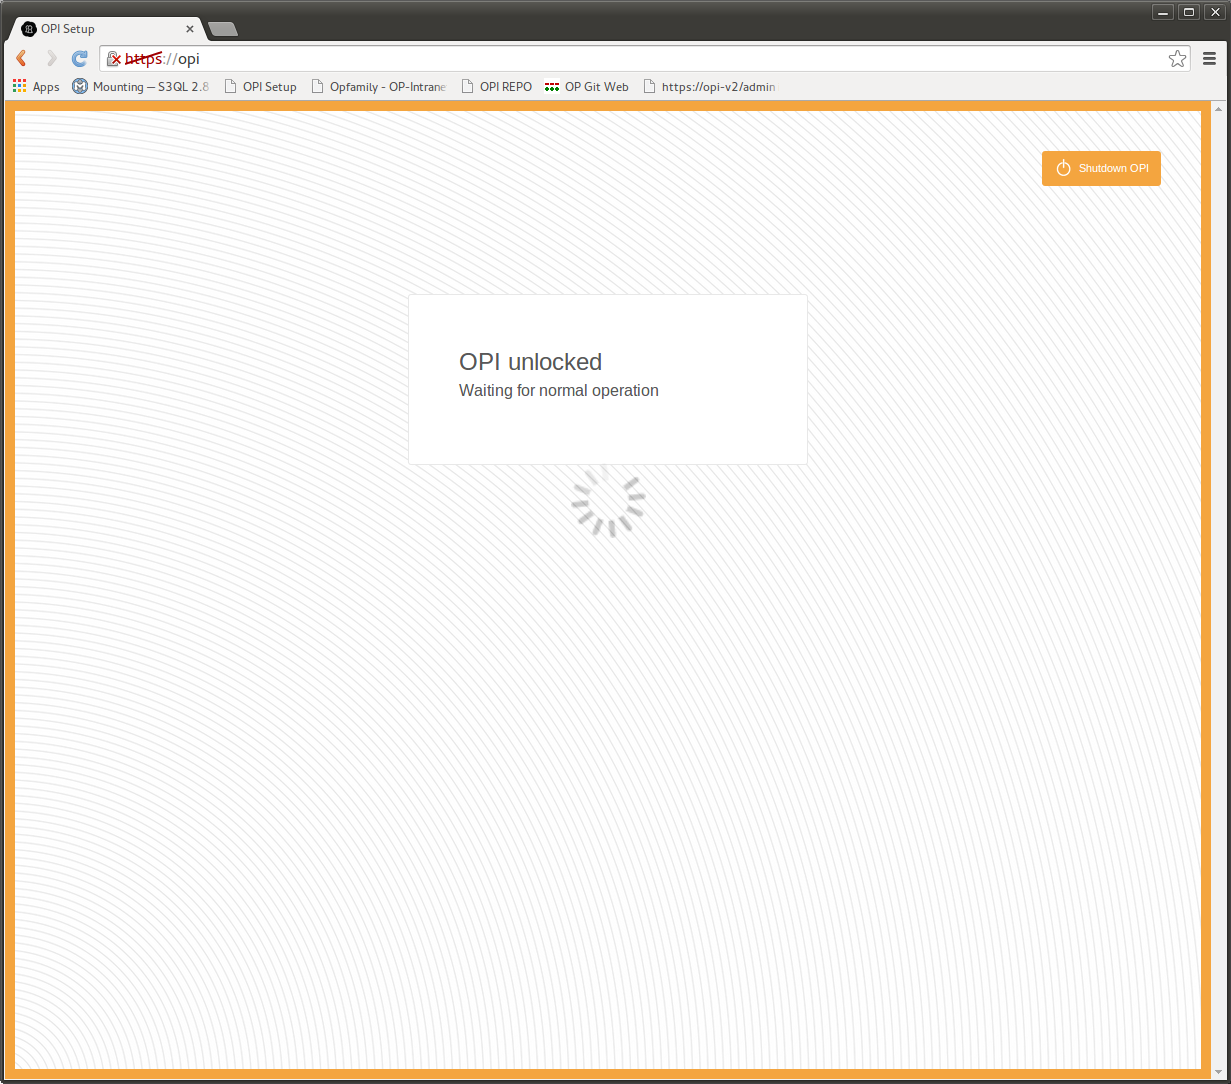
\includegraphics[width=10cm]{./img/unlocked}
\caption{KEEP has been unlocked and starting services}
\end{figure}
KEEP has been unlocked and is starting all services and will redirect to the login page.
During this step, KEEP has downloaded a certificate that has been created by KEEP and signed by OpenProducts servers.

When redirecting to the login page, you will be warned that the certificate that was just generated is not trusted. This warning is expected and can be safely ignored.

The process of adding the certificate, or OpenProducts CA (certificate authority) differs between browsers, please see the FAQ on our  \href{http://community.openproducts.com}{forum}. 

\newpage
\subsection{Sign In}
Sign into your KEEP with your newly created username and password. 
\begin{figure}[h!]
\centering
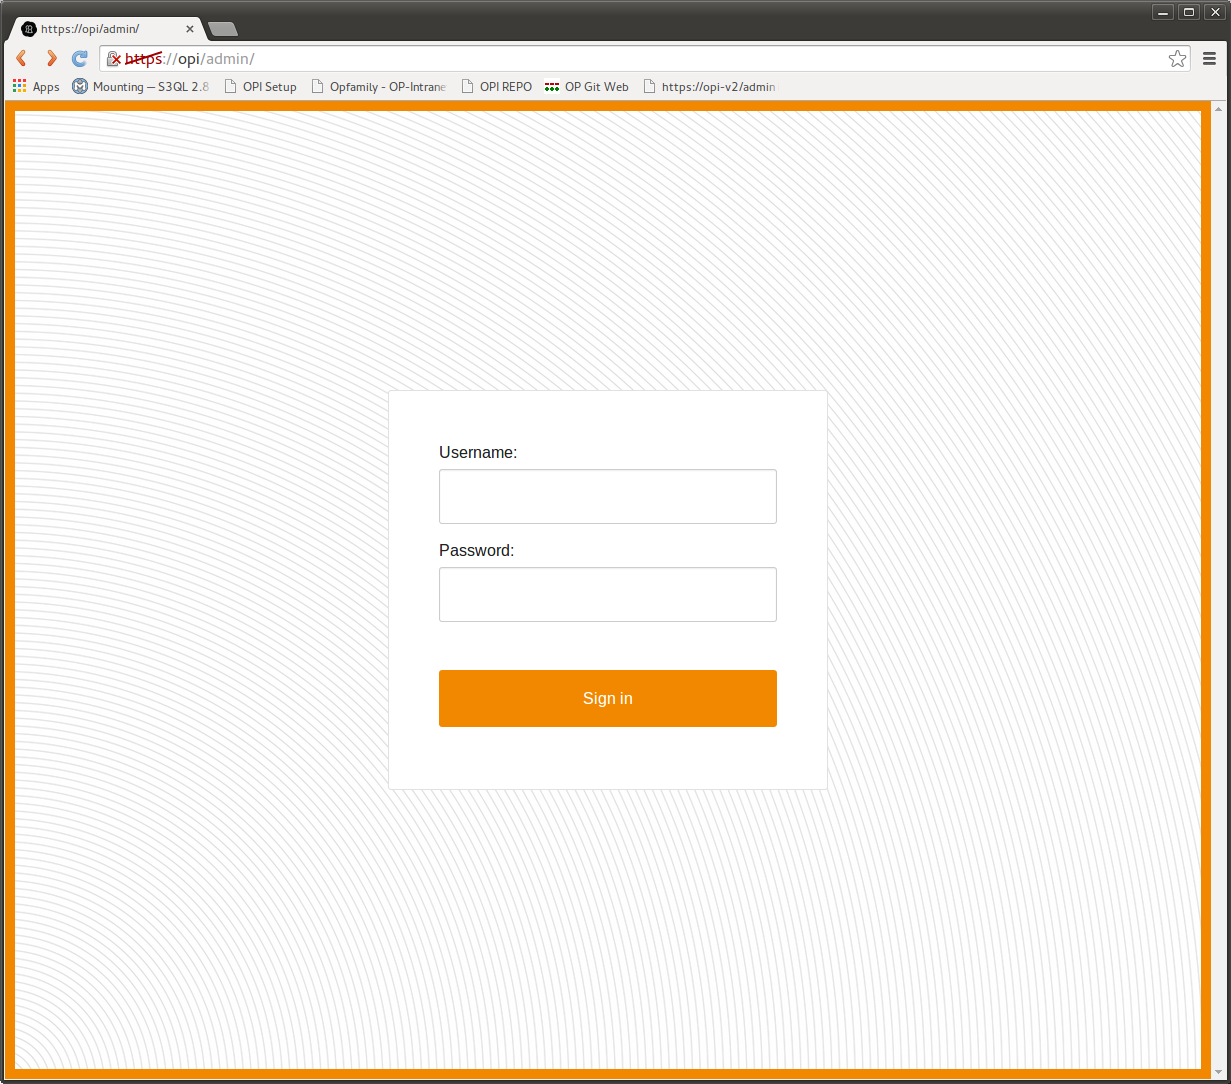
\includegraphics[width=10cm]{./img/sign-in}
\caption{Sign in to KEEP}
\end{figure}

\newpage
\subsection{Navigation Between Applications}
In order to quickly be able to switch from one application to the next, a menu system is available in the top right corner of the web interface.

By clicking the orange boxes, a drop down menu is activated and the different applications are presented. 

\begin{figure}[h!]
\centering
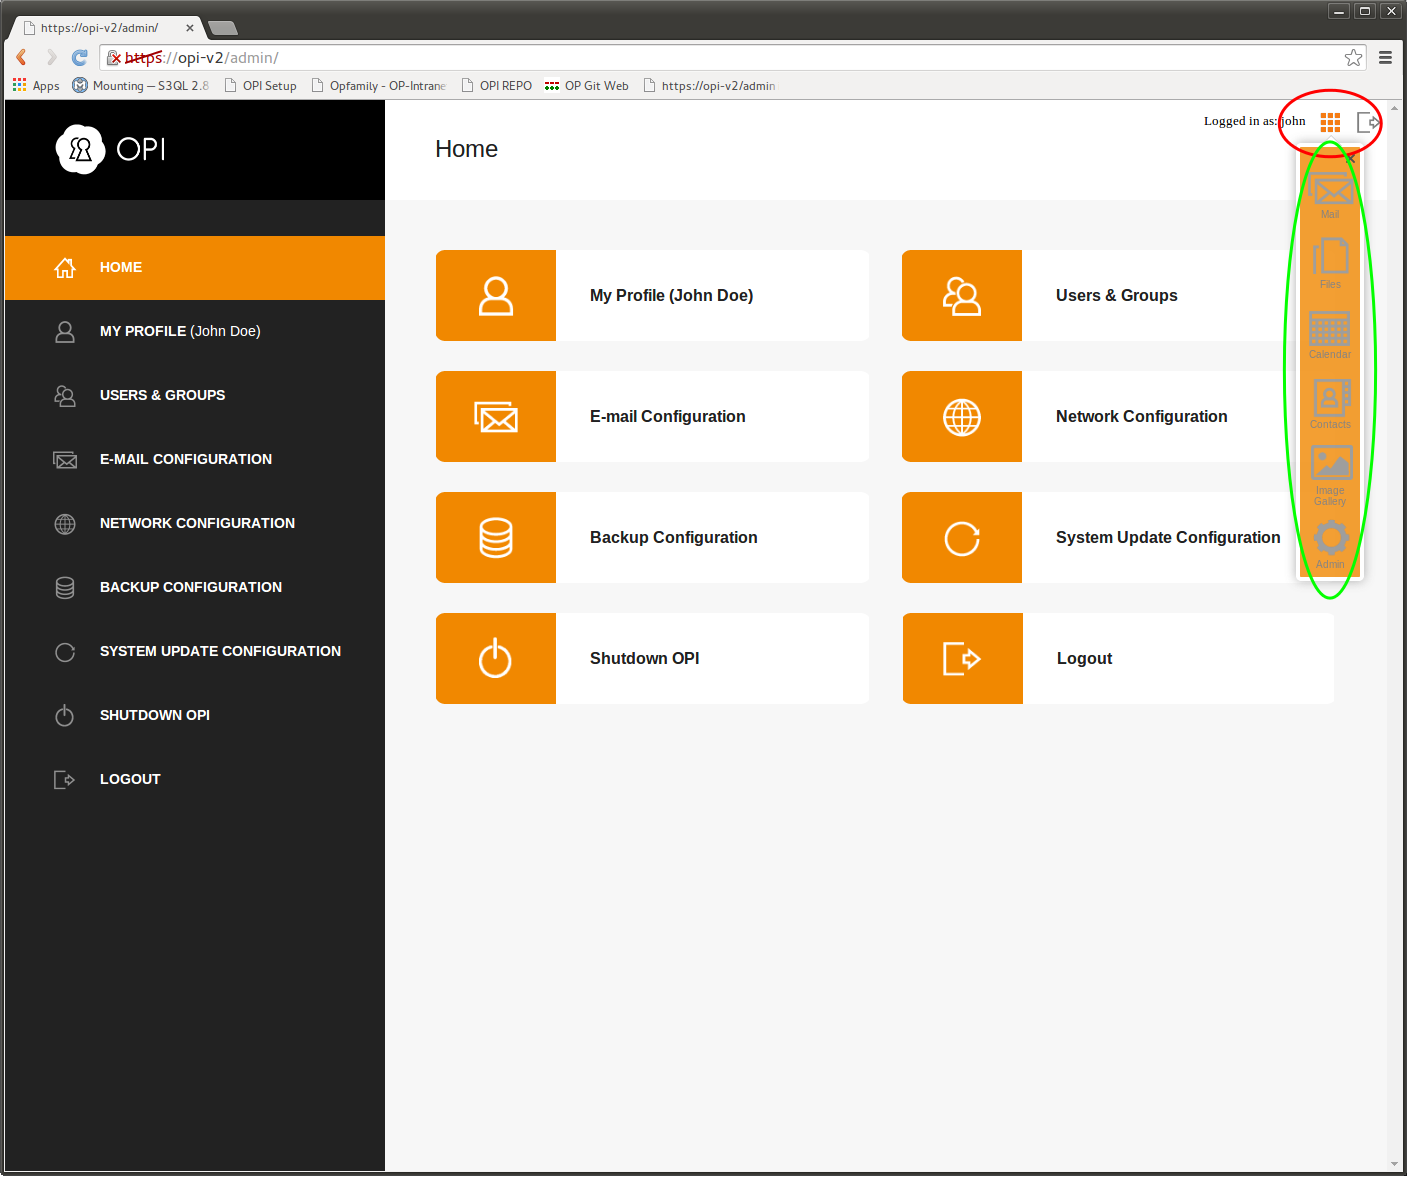
\includegraphics[width=10cm]{./img/menu-admin}

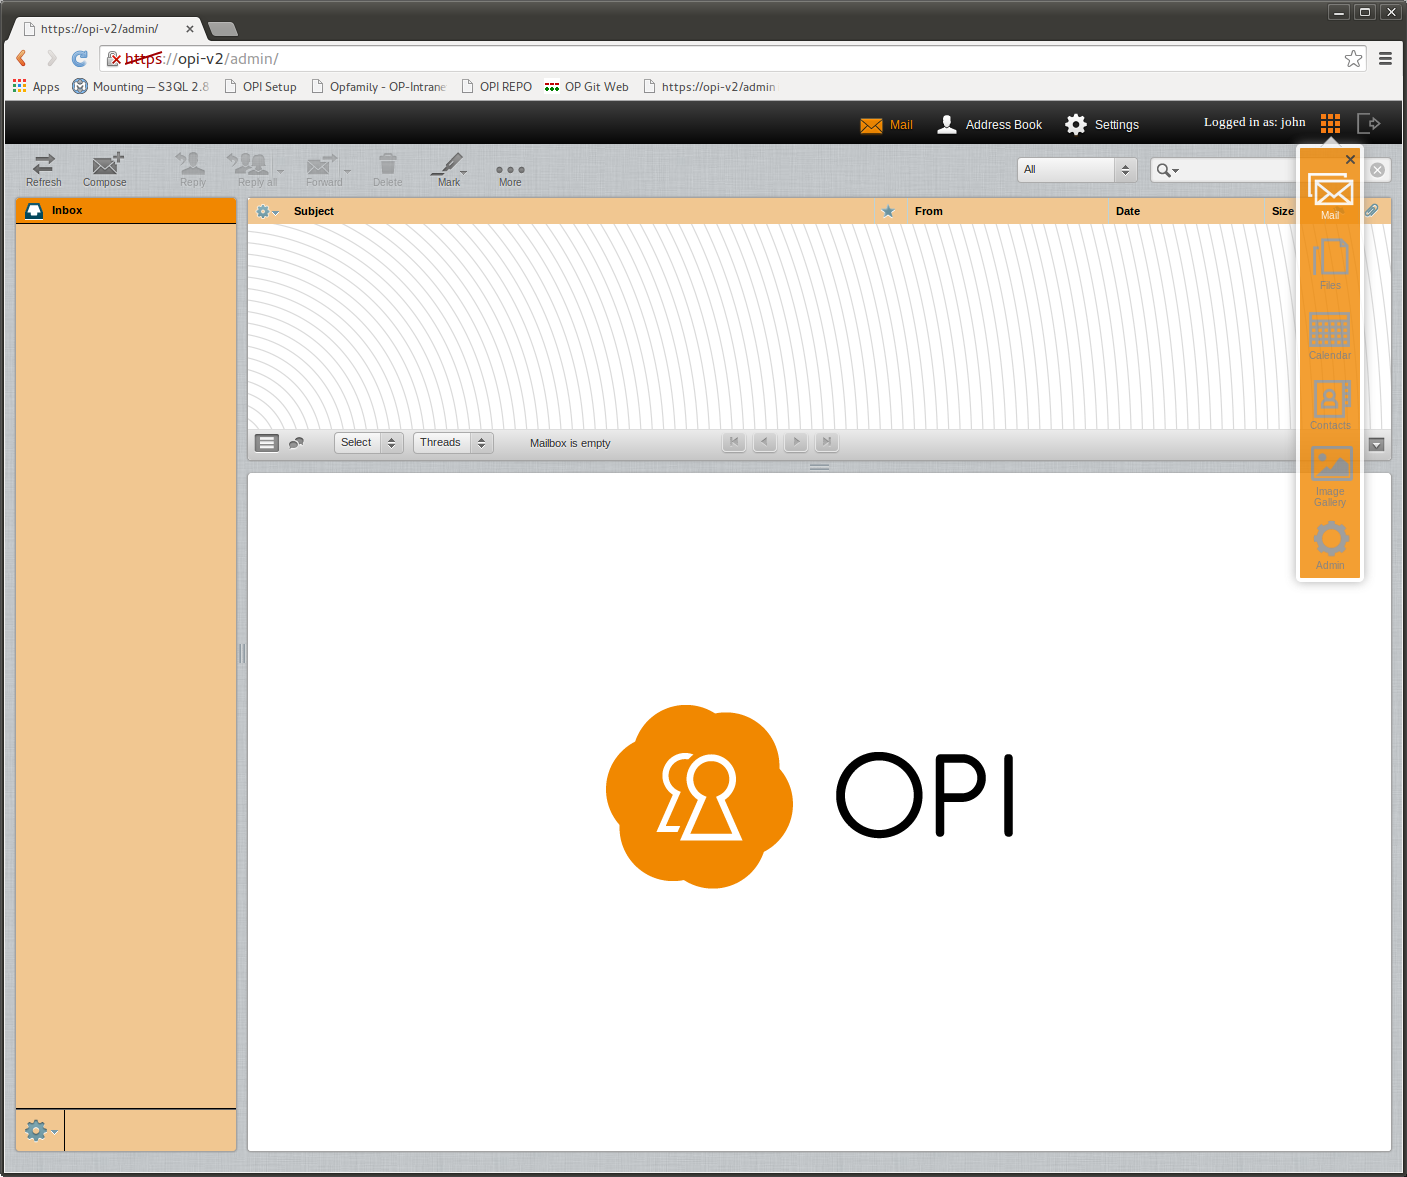
\includegraphics[width=4.93cm]{./img/menu-mail}
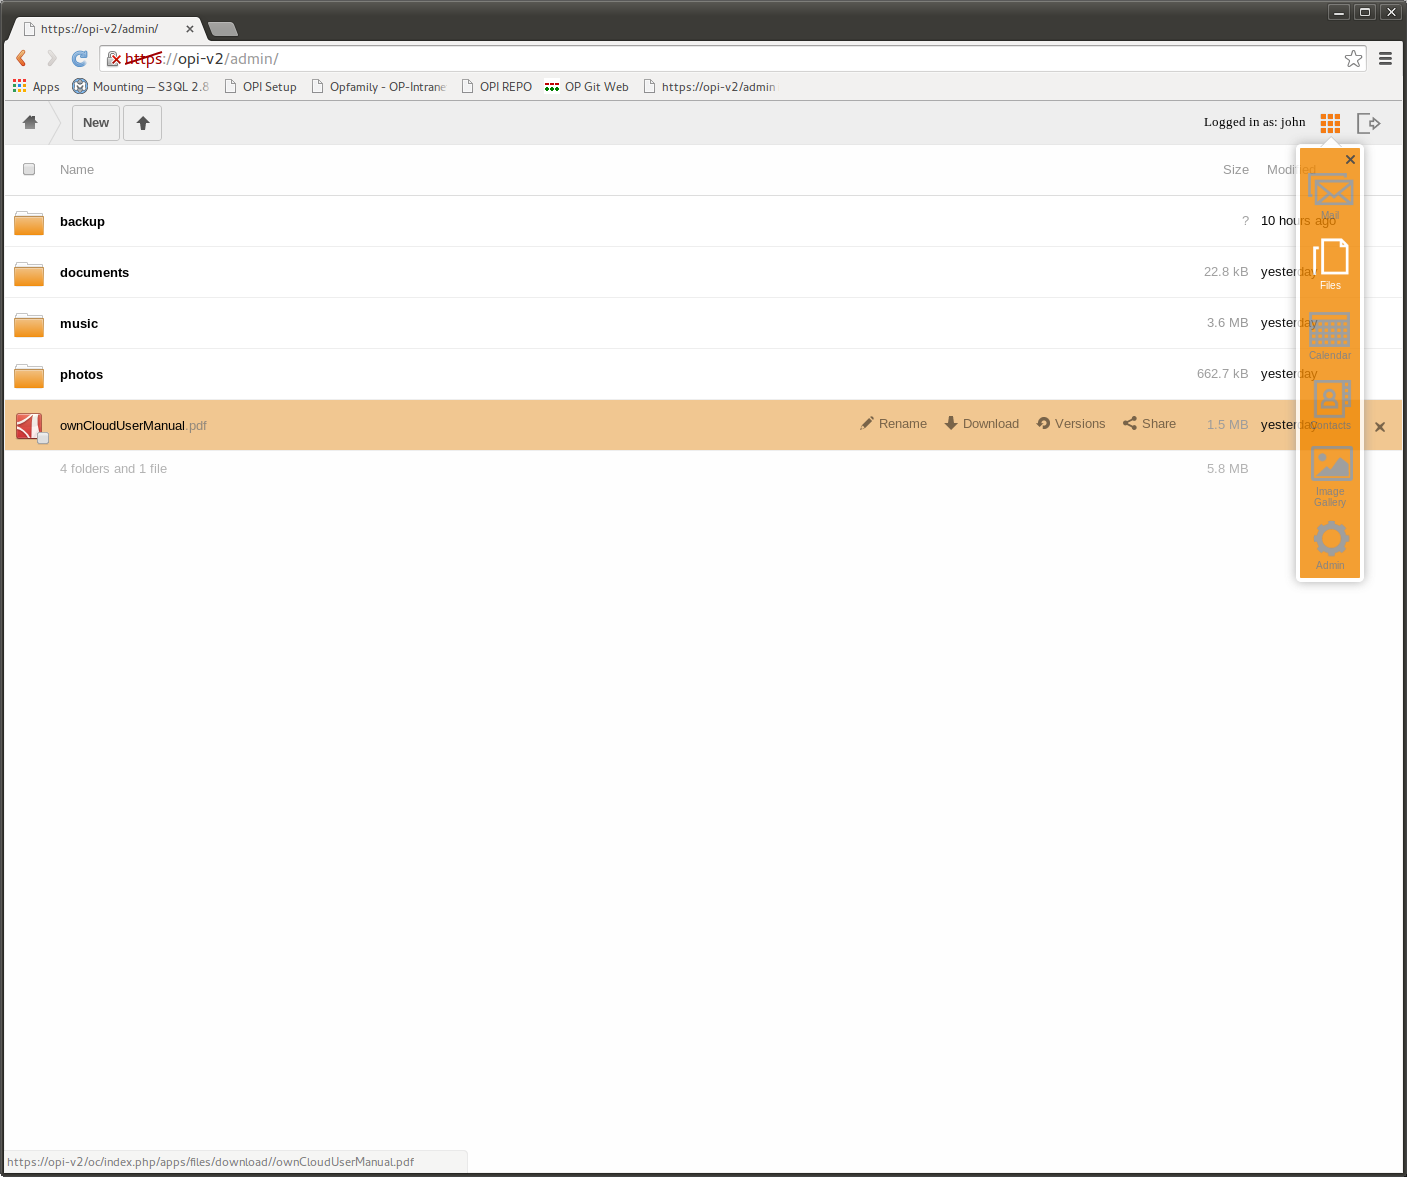
\includegraphics[width=4.93cm]{./img/menu-files}
\caption{Use the quick menu to access the different applications}
\end{figure}

\newpage
\subsection{LEDs}
On the front of KEEP there is one LED.
The following table describes the meaning of these.
\begin{table}[h!]
\centering
\renewcommand{\arraystretch}{1.5}
\renewcommand{\tabcolsep}{0.2cm}
\begin{tabular}{|c|c|c|l|}
\hline
\textbf{LED}&\textbf{Meaning} \\
\hline
Solid Green & Normal Operation \\
\hline
Solid Blue & Initial System Startup \\
\hline
Blue Heartbeat & Linux is booting\\
\hline
Green Heartbeat & System is avaiting input or Backup is ongoing \\
\hline
red & Something is wrong, check the admin UI for details. \\
\hline
\end{tabular}
\caption{LED interpretation}
\end{table}

\newpage
\section{Recommended Extended Setup}
\subsection{Enable Backup}
To secure your data we recommend that you enable backup of your data. Not only does this protect you of data loss in case of theft or hardware malfunction, it also provides a time line of your data making it possible to retrieve data from previous versions even if the current data is changed.
\begin{itemize}
\item Login with an administrative account (the first user account created during setup is automatically created as an administrative account).
\item Select ``Backup configuration''
\item Check the box ``Enable backup''
\item Select either ``OpenProducts Servers'',  ``Amazon S3'' or ``Local'' target
\end{itemize}

\begin{figure}[h!]
\centering
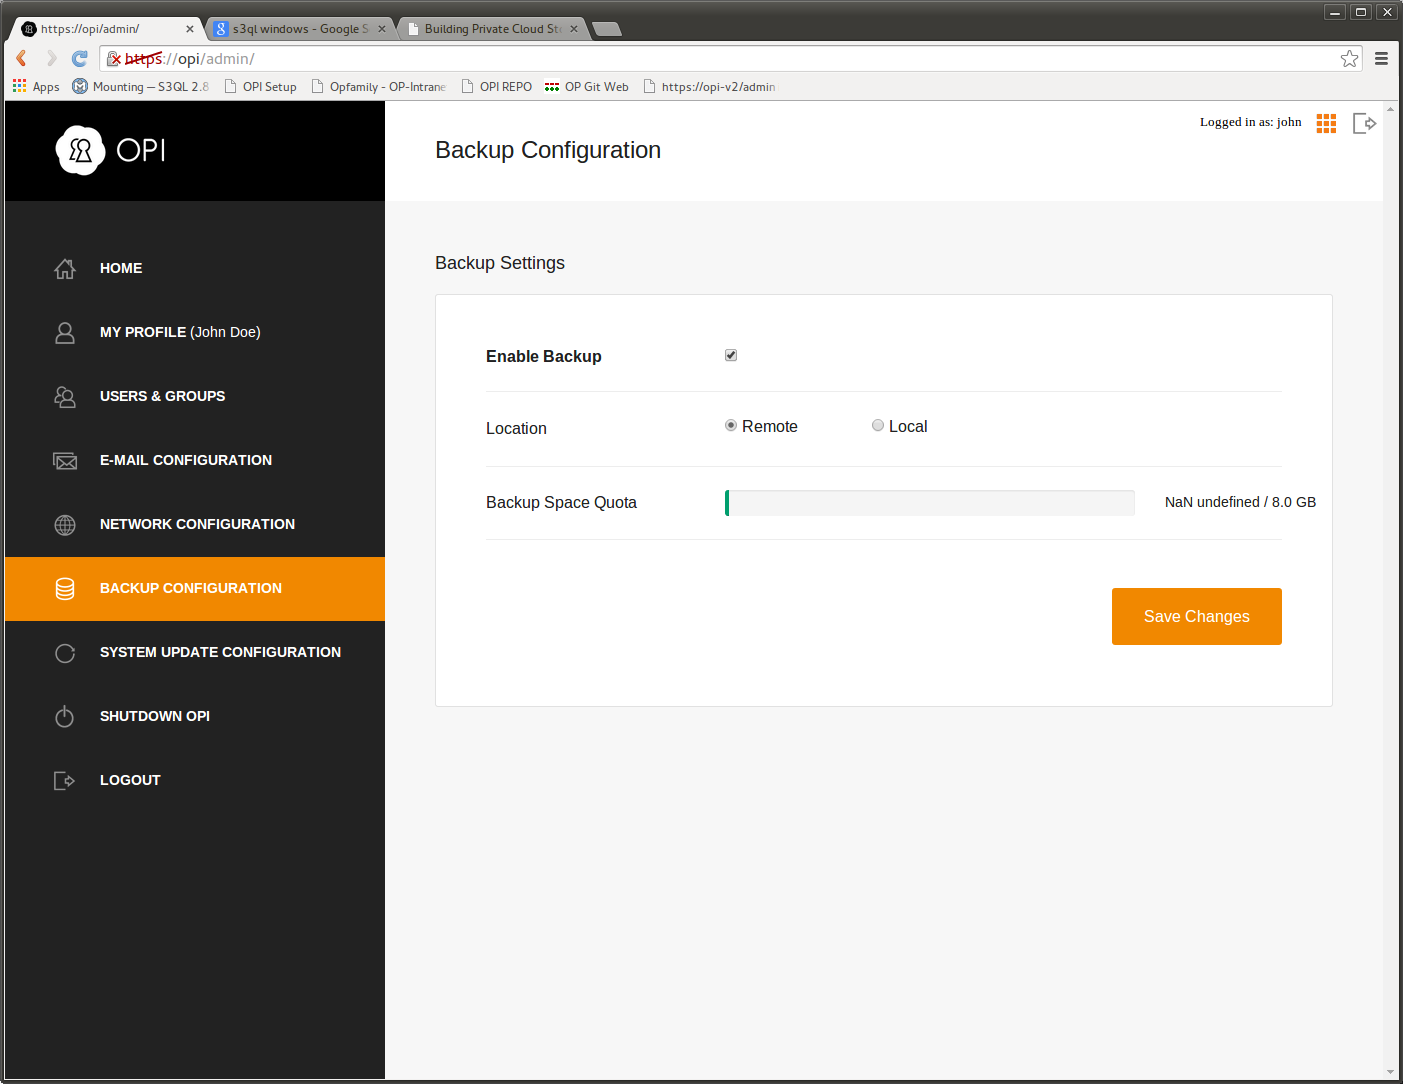
\includegraphics[width=10cm]{./img/backup_config}
\caption{Backup configuration}
\end{figure}

The ``OpenProducts Servers'' target is OpenProducts servers, located in Sweden. By default, all users are granted 8GB space on our servers free of charge for 3 months.

To ``Amazon S3'' target you need to supply an existing bucket, the ``Amazon Access Key'' and the ``Amazon Secret Access Key'' to access the S3 account. \href{http://www.ezs3.com/public/231.cfm}{Read here how to find them}.

In order to use the ``Local'' target, a USB memory or disk needs to be inserted in the USB port on KEEP. That device will then be used for backup.

Note that all backups are encrypted prior to leaving KEEP, meaning that no one that does not have your master password has the possibility to decrypt your information.
Also note that currenlty the Amazon backend is not supported during a total re-install. The data will be accessible after the re-install, but all users and system settings have to be manually entered.

\subsection{Mail Setup}
\subsubsection{Mail Server Configuration}
In order to have mail working properly a few things need to be setup.

If your ISP (Internet Service Provider) allows you to send mail directly, then KEEP will try to deliver any mail sent from the system directly to the recipients mail server. If this is the case, then select "Use KEEP to send mail".\\
However, even if KEEP is allowed to send the mails, it is not sure that the receiving mail server will accept the message. This is due to the amount of spam today, and many mail servers requires that the sending mail server must be in various ``white lists'' or else the email will be rejected.

\begin{figure}[h!]
\centering
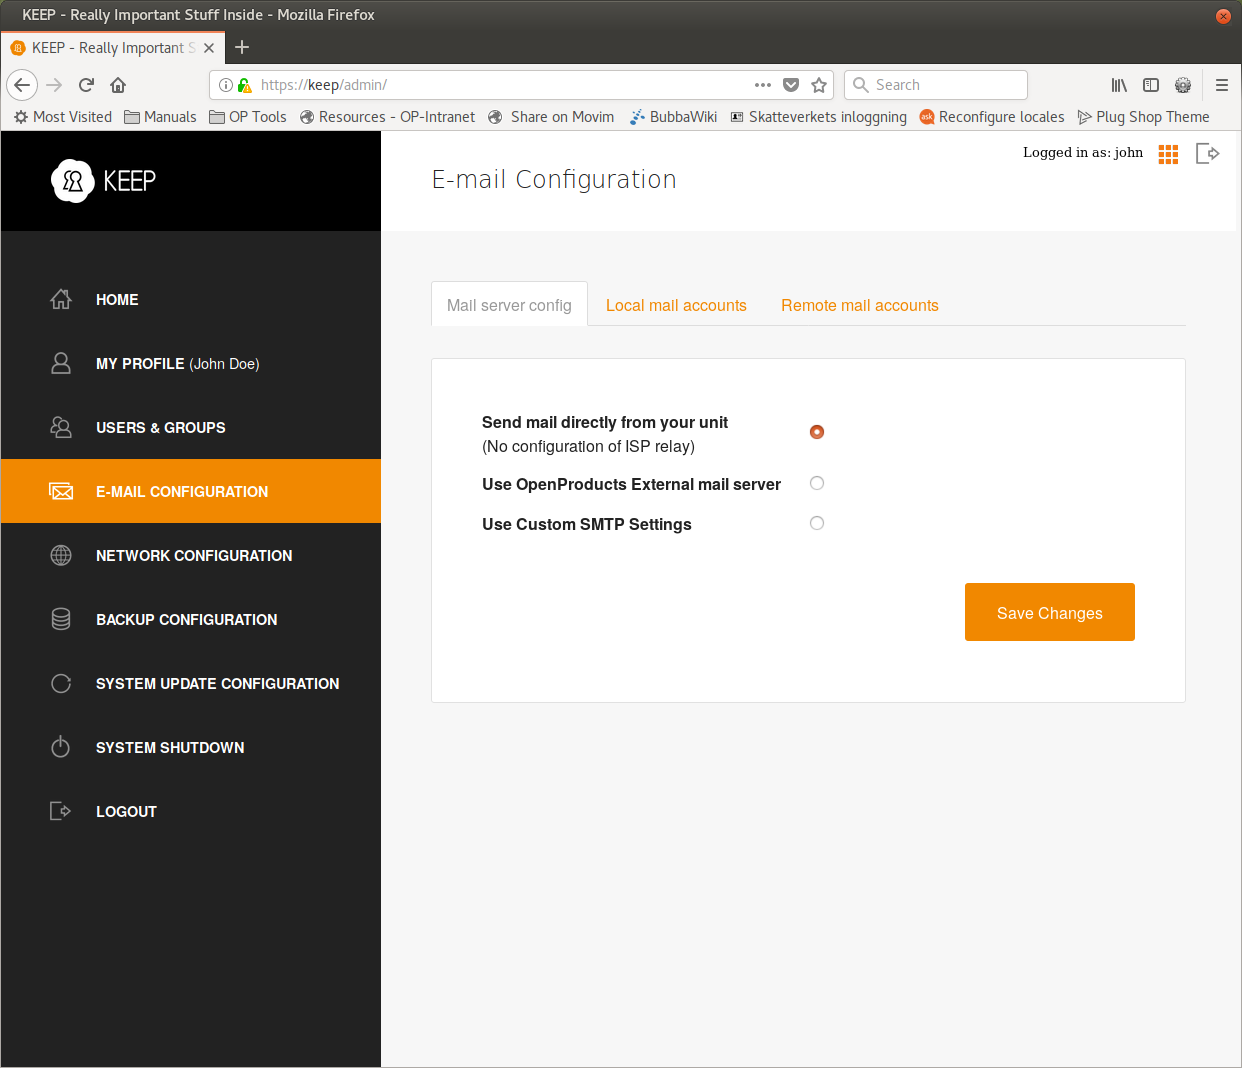
\includegraphics[width=10cm]{./img/smtp_config}
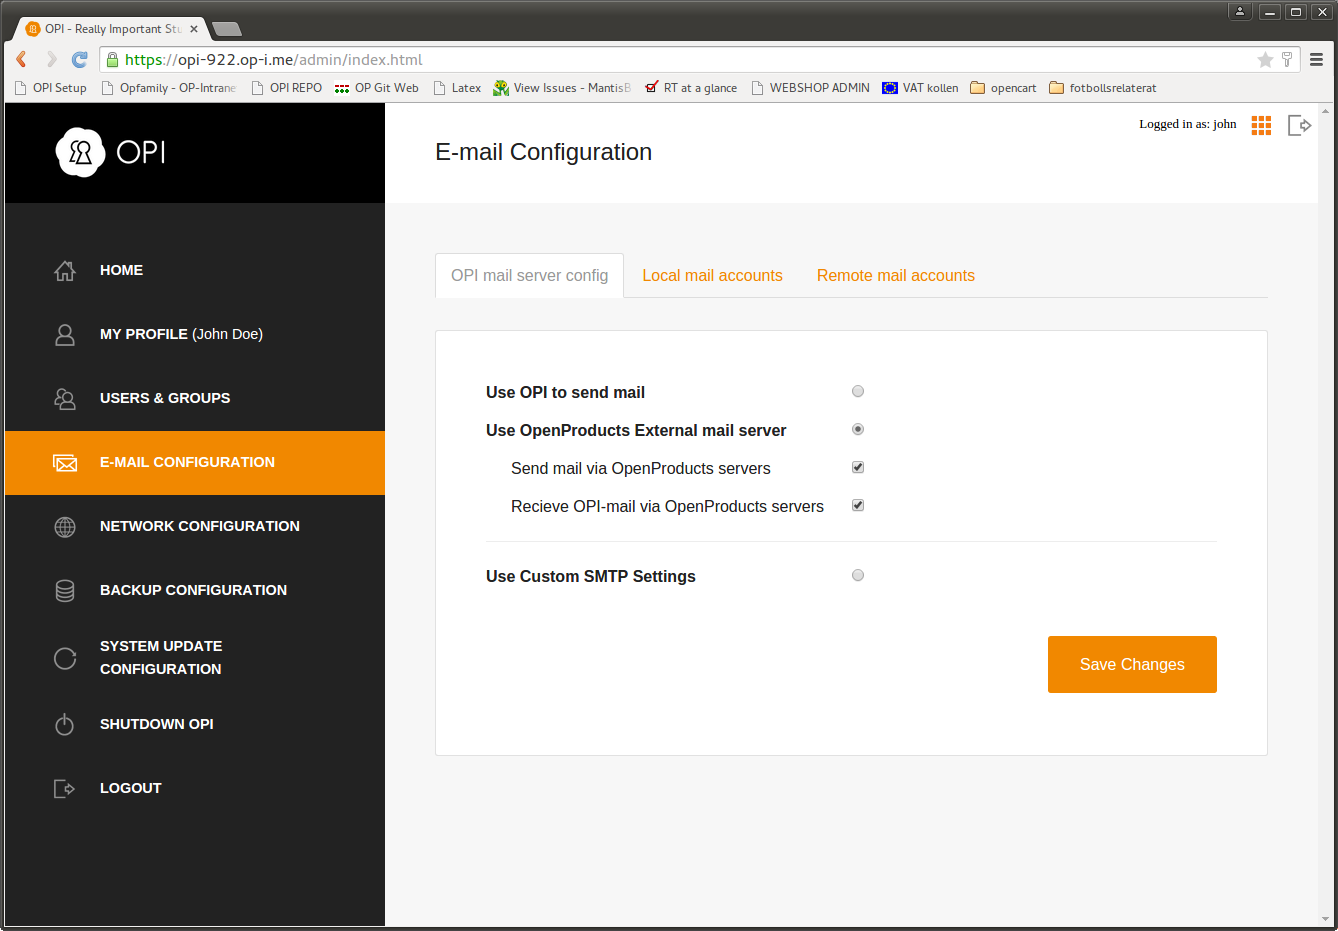
\includegraphics[width=4.93cm]{./img/smtp_config-2}
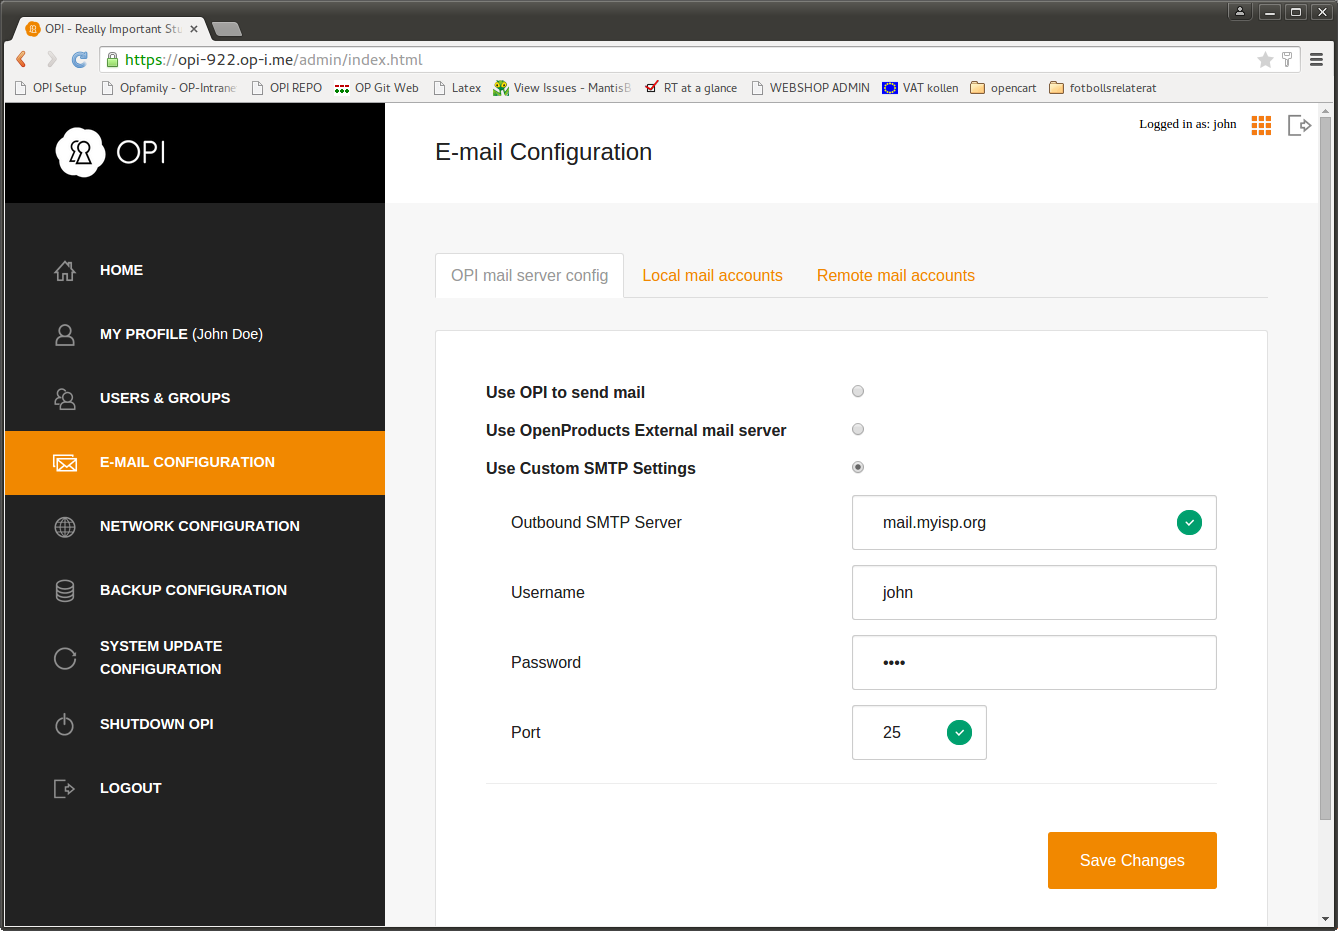
\includegraphics[width=4.93cm]{./img/smtp_config-3}
\caption{Mail configuration}
\end{figure}
The next possibility is to use a relay server. This means that KEEP will contact a server that is allowed to send mail.

OpenProducts does provide such server to be used by KEEP-devices. This can be selected by checking the "Use OpenProducts External mail server" option. This will in turn offer the selection to use our servers for either incoming and/or outgoing mail.

Using the OpenProducts Relay server for incoming mail also requires that port 2525 is open (forwarded) to your unit and available from the internet. The intention of this configuration is to allow mail to be received even if the ISP blocks port 25, which is fairly common.

The third option will allow to specify custom server details, this is what should be used if you need to fill in your ISP's outgoing mail server (known as SMTP server) configuration. By selecting this option, a form where the details about the server can be entered.


\subsubsection{Receiving Mail}
By default, KEEP will be setup to accept incoming emails sent to all users created on the system. For these accounts, the email address used is in the form of ``username@devicename.mykeep.net''. In the section ``E-mail Configuration -\textgreater Local mail accounts'' it is possible to add additional addresses, including mail addresses that are on domains pointing to KEEP.\\
If other domains are added, the recommended setup is that the MX pointer is set to devicename.mykeep.net, since that IP address is updated by KEEP.
\begin{figure}[h!]
\centering
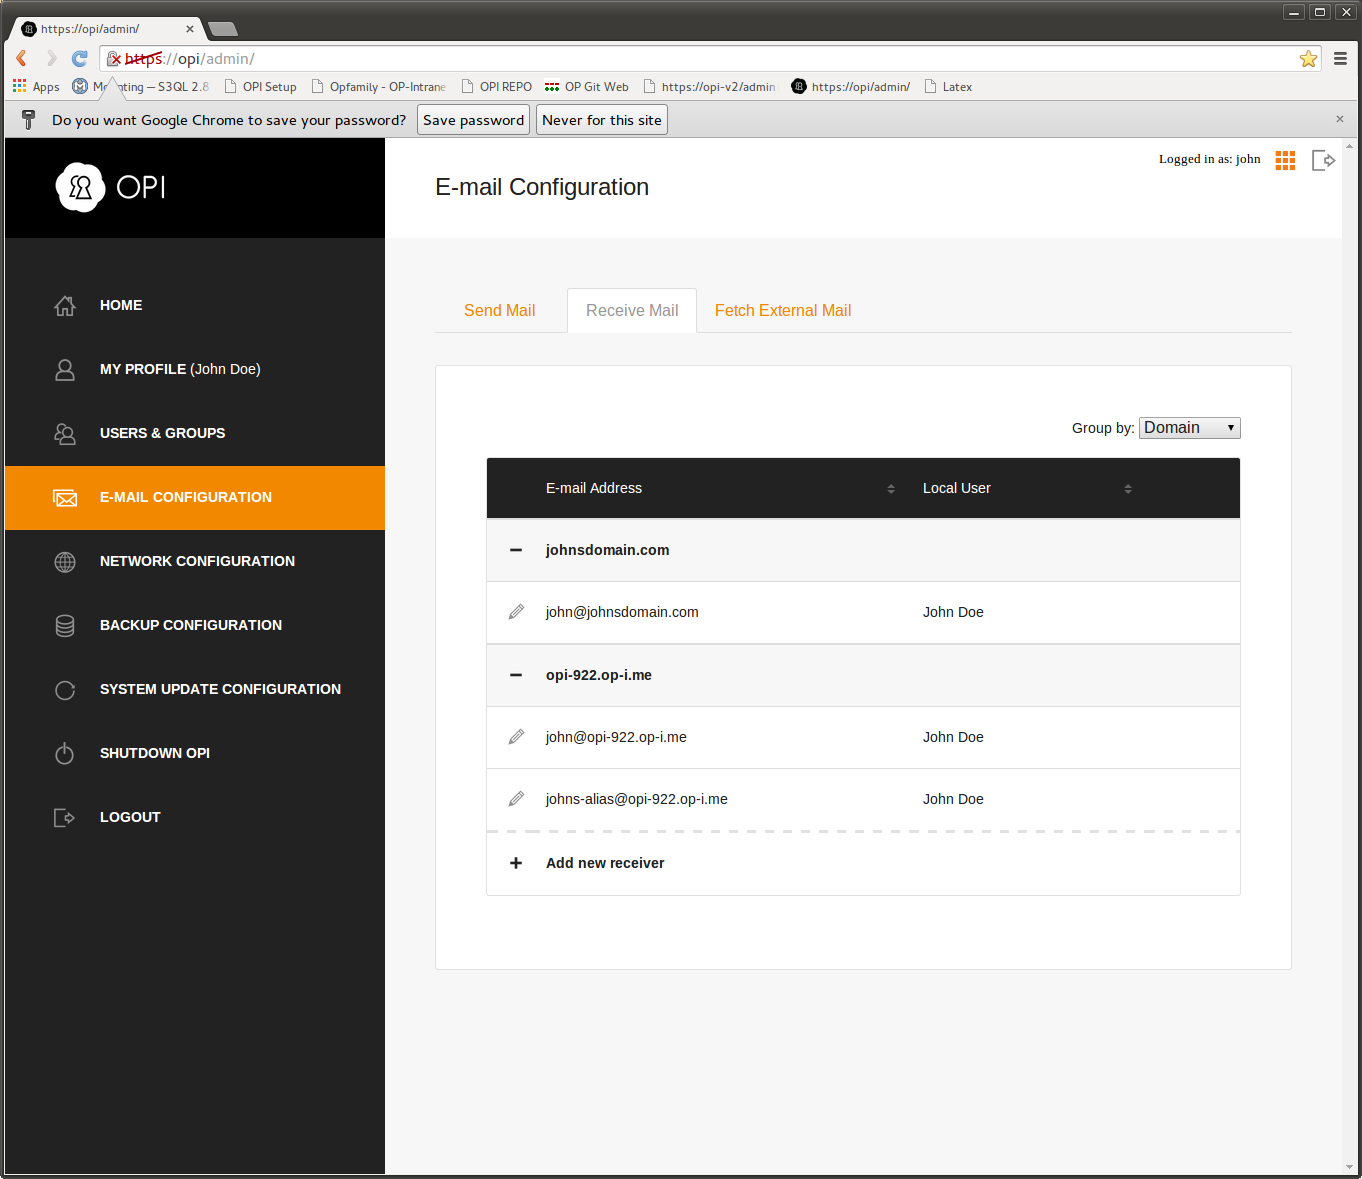
\includegraphics[width=10cm]{./img/receive-mail}
\caption{Receive mail configuration}
\end{figure}

It is possible to group addresses either by local user or by domain by the drop down box.

\subsubsection{Remote mail accounts}
In order to collect all email in one location, it is possible to set up KEEP to fetch mail from external accounts such as GMail or from other providers. Currently GMail accounts need to have the "\href{https://support.google.com/accounts/answer/6010255?hl=en}{Less Secure Apps} enabled to allow access for KEEP to retreive mail.
In the section ``E-mail Configuration -\textgreater Remote mail accounts'', by clicking ``Add external mailbox'' remote accounts are added from which KEEP will retrieve mail.
Depending on if the configurations can be figured out automatically different fields will be visible during configuration.
\begin{figure}[h!]
\centering
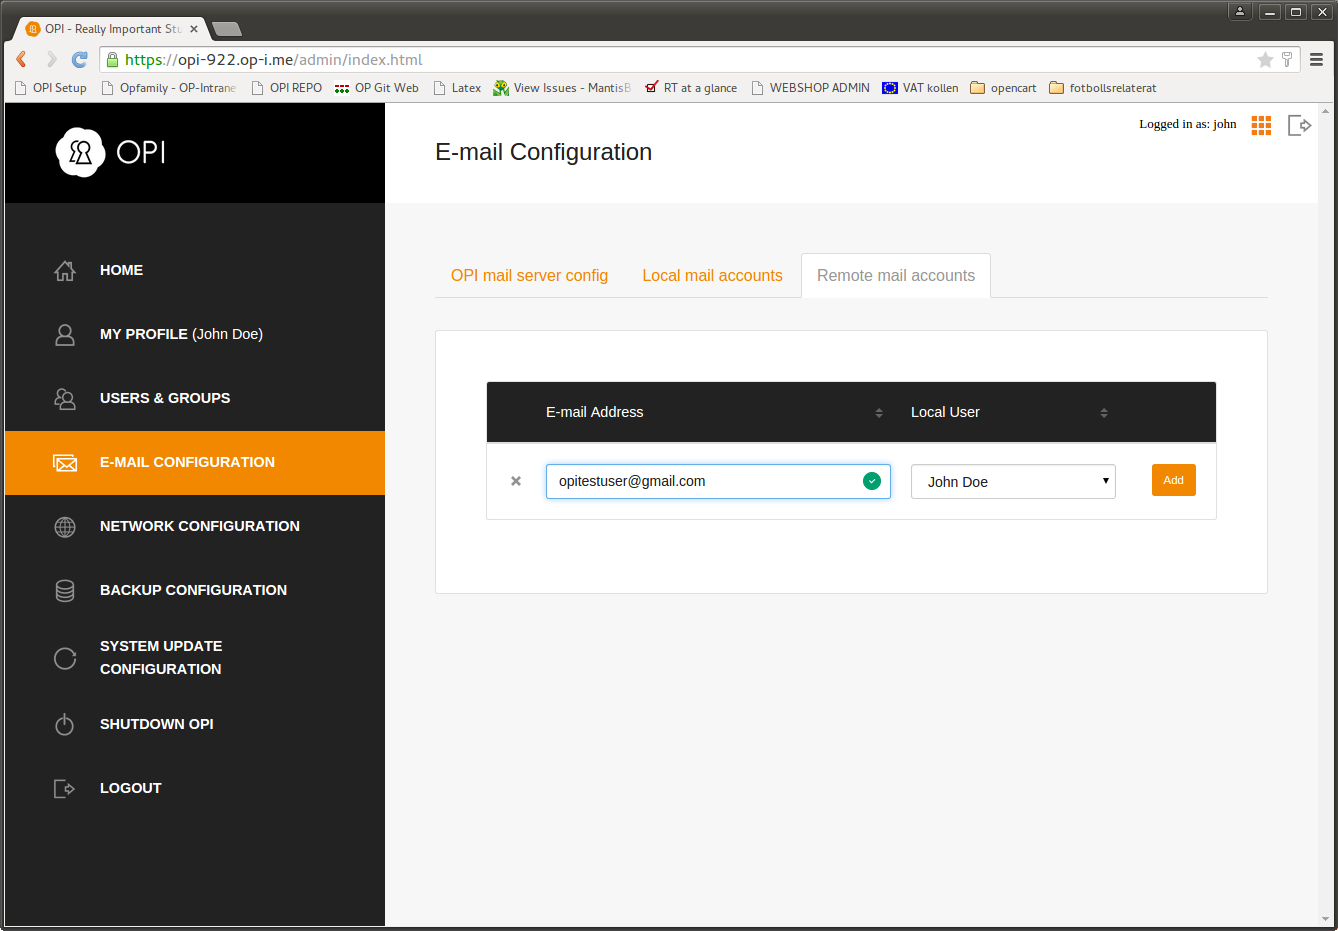
\includegraphics[width=10cm]{./img/fetch-mail-1}

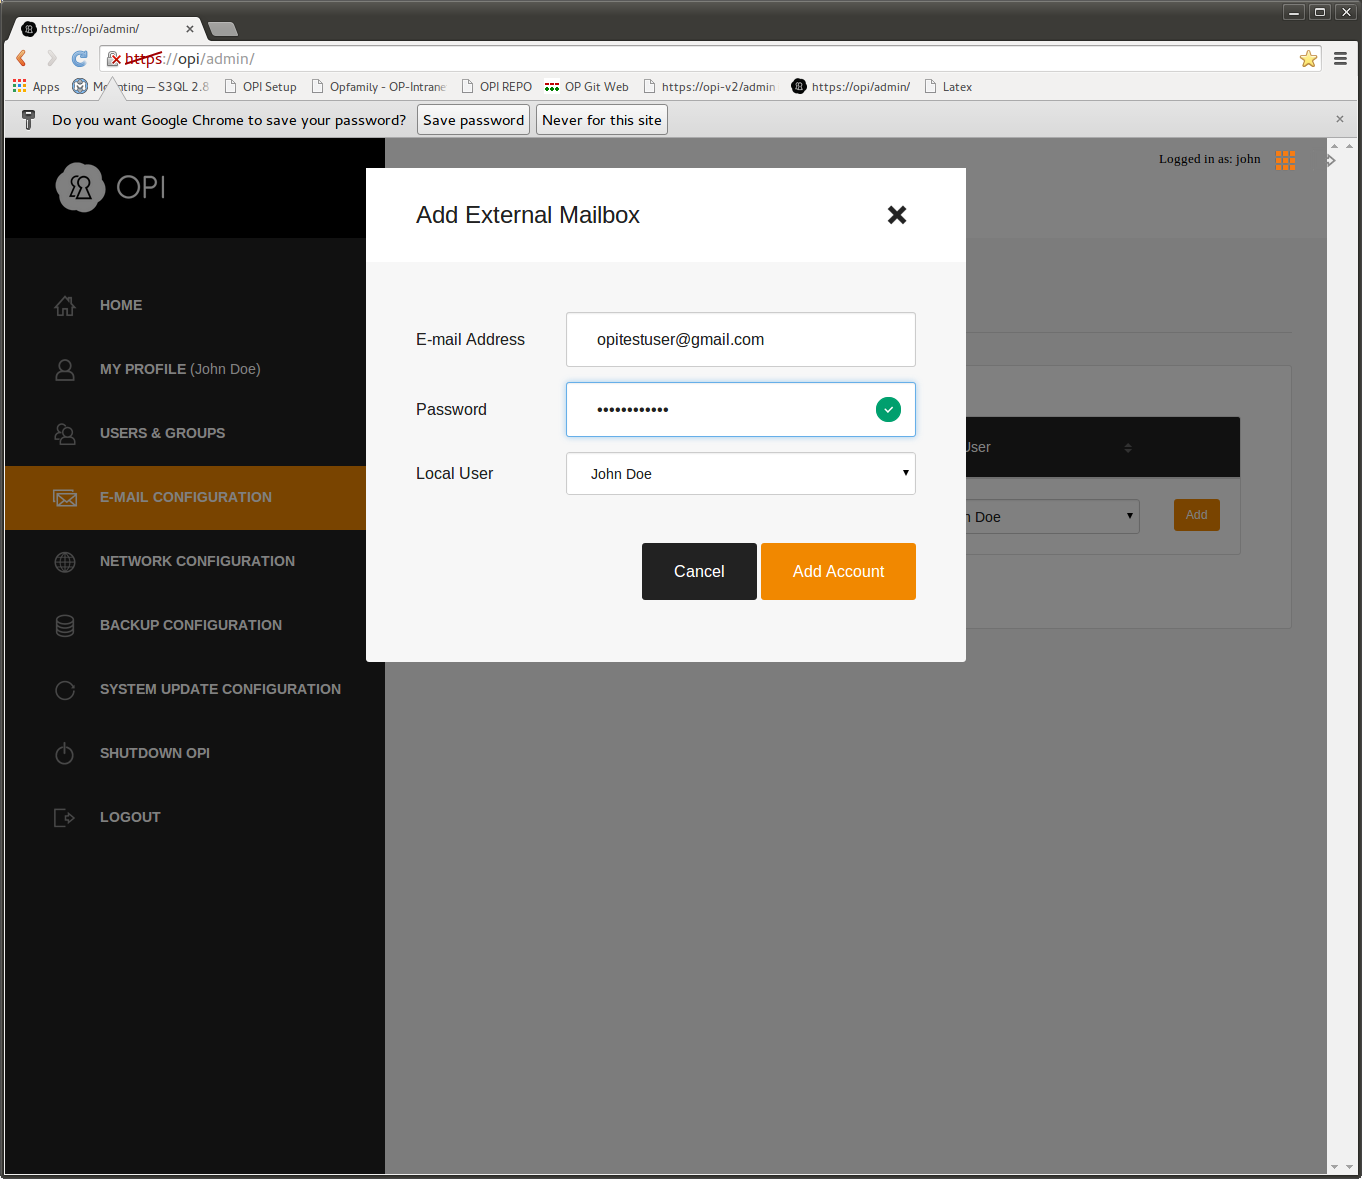
\includegraphics[width=4.93cm]{./img/fetch-mail-2}
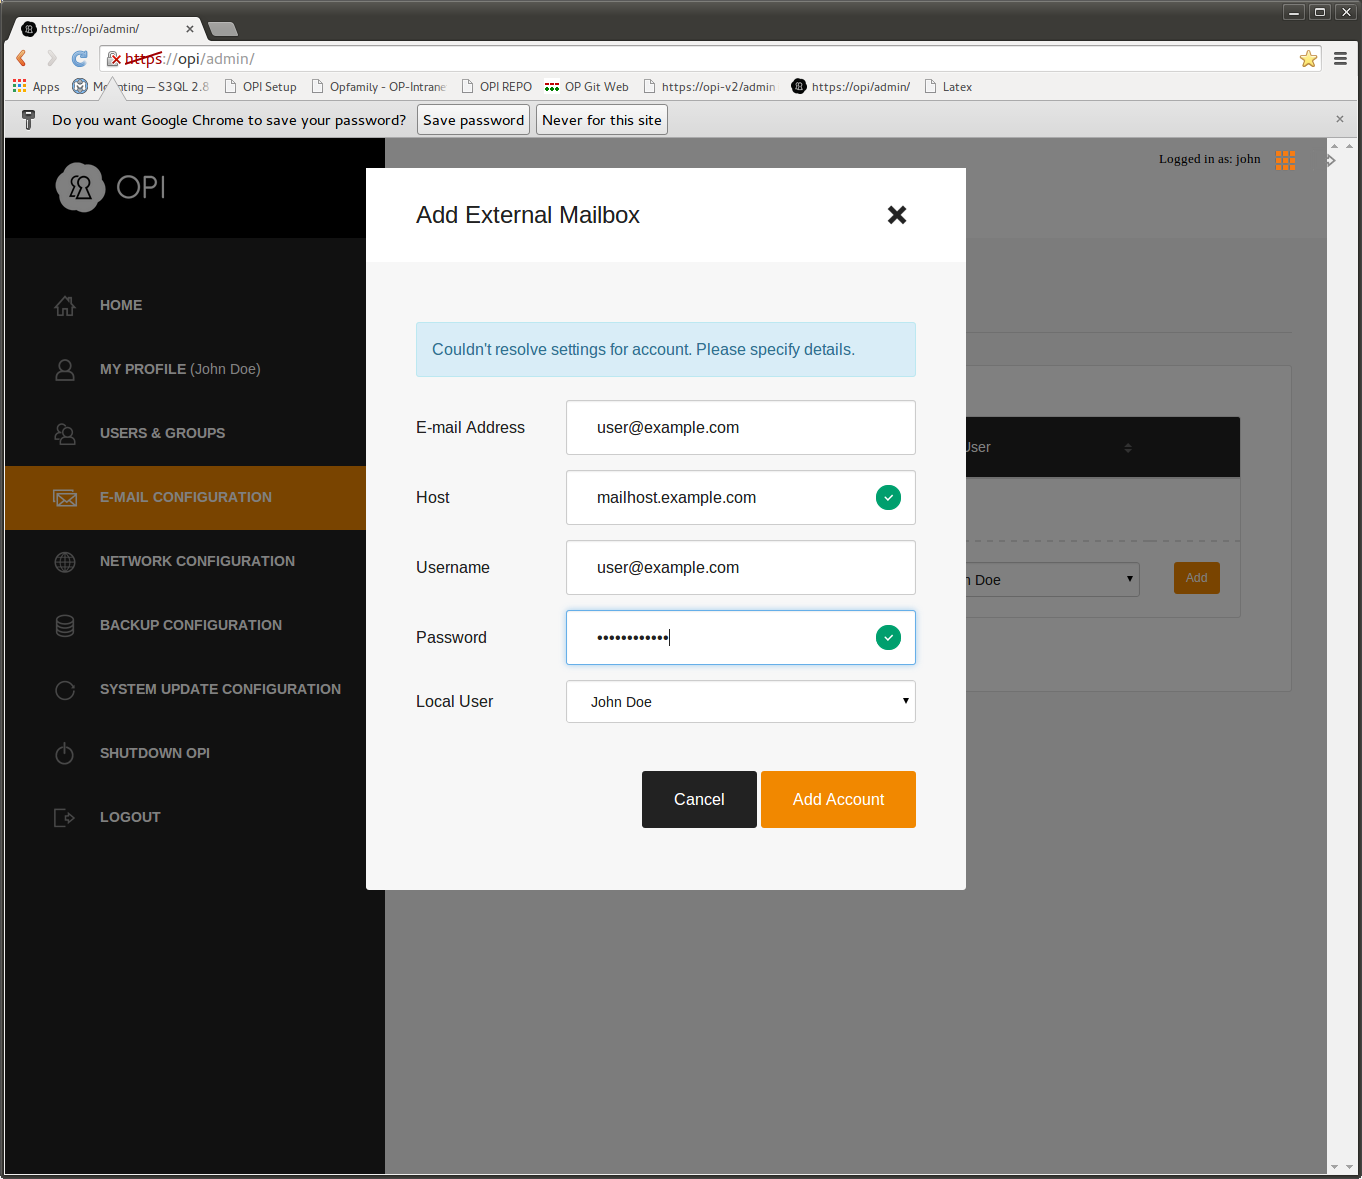
\includegraphics[width=4.93cm]{./img/fetch-mail-3}
\caption{Fetch external mail configuration}
\end{figure}

\subsection{Users and Groups}
All user and group management is common for all applications in the system and managed from the ``Users \& Groups'' section.
\subsubsection{Adding users}
Users are added by clicking ``Add users'' and entering the user details. A dialog box is then presented to enter the users password.

All users can be edited by clicking the pen icon on the relevant user, then selecting the appropriate action.
\begin{figure}[h!]
\centering
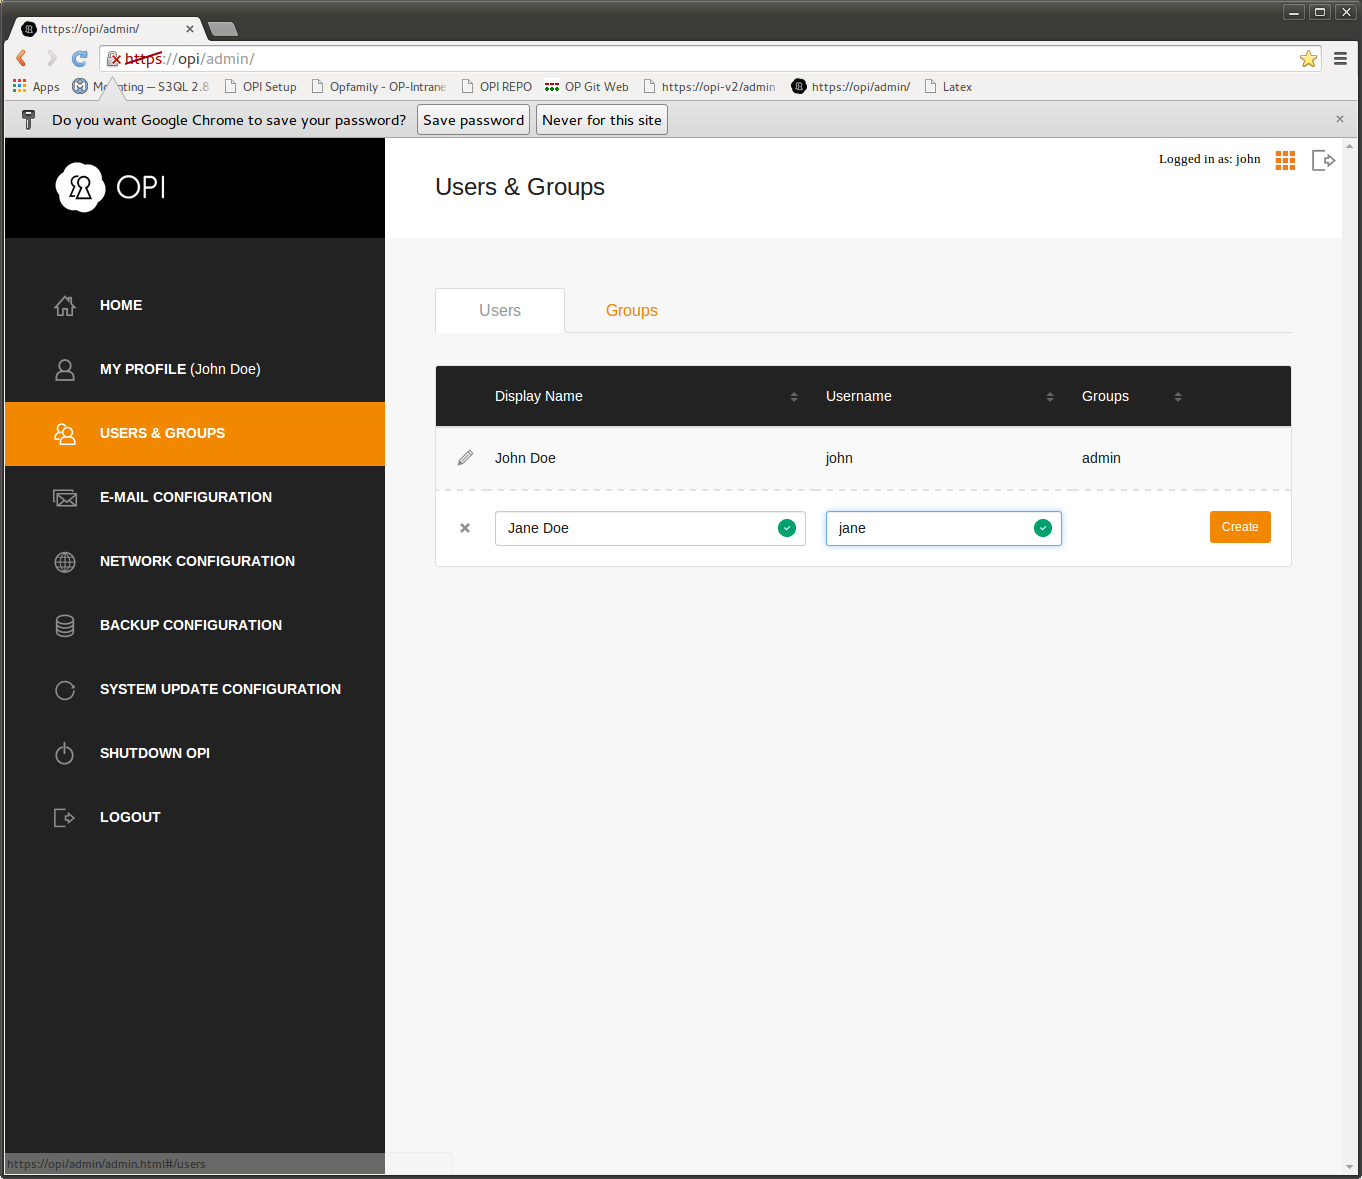
\includegraphics[width=4.93cm]{./img/users-1}
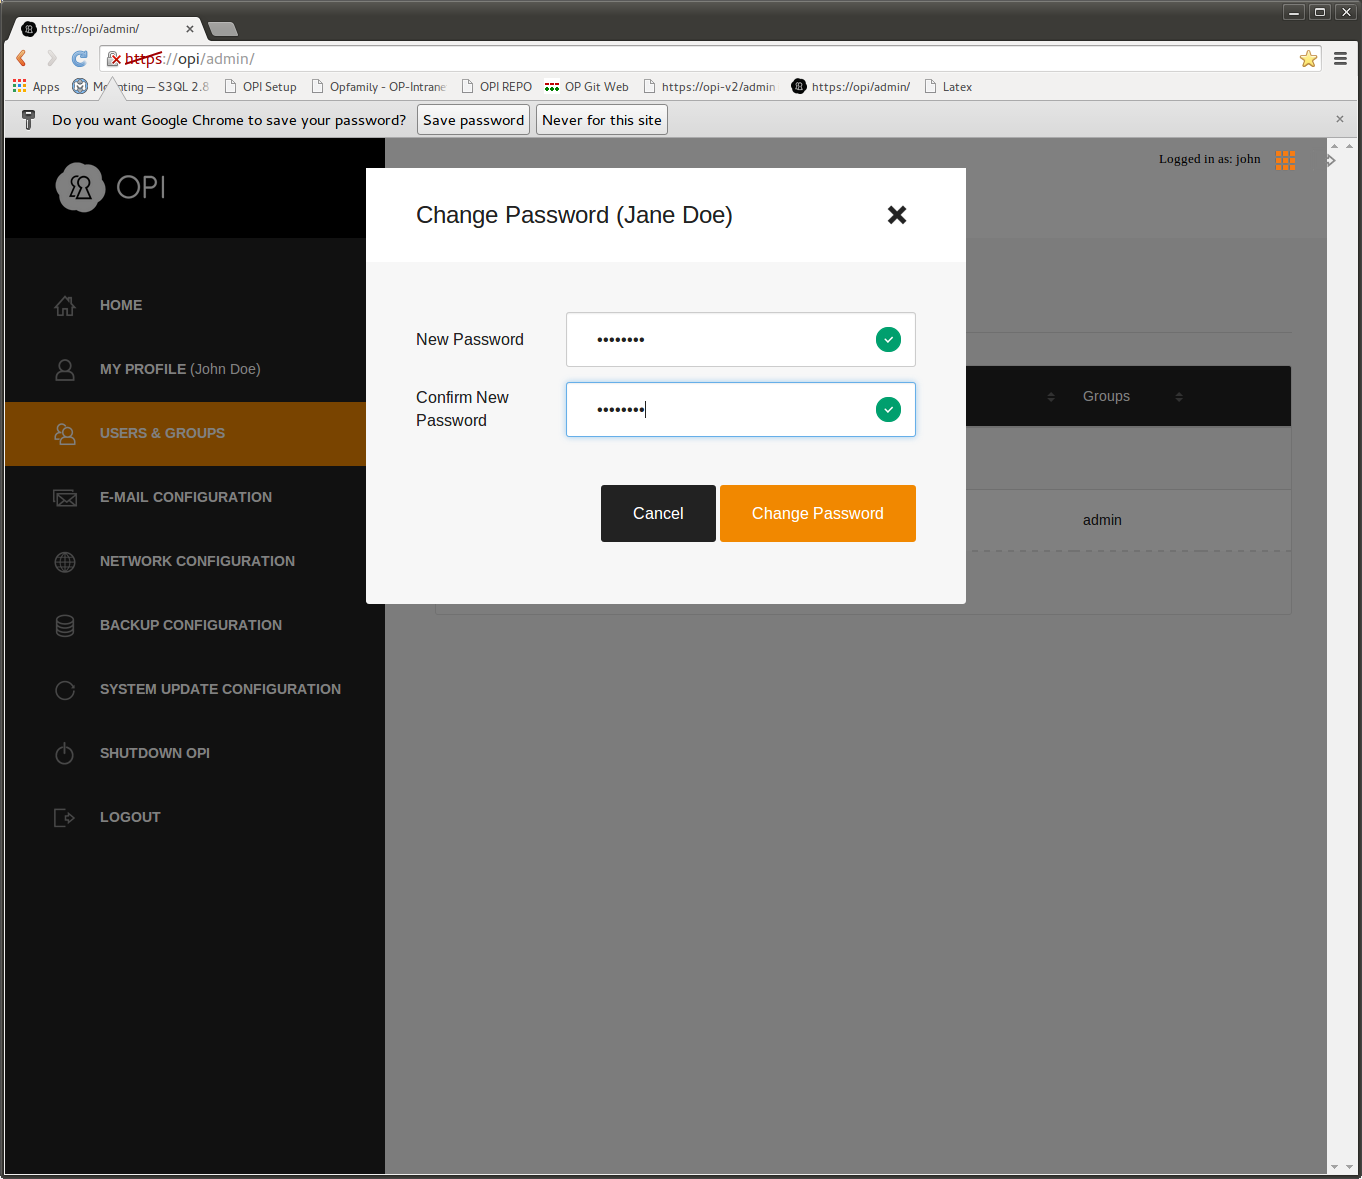
\includegraphics[width=4.93cm]{./img/users-2}
\caption{Adding users}
\end{figure}

\subsubsection{Adding Groups}
Groups are added much in the same way as users. Groups can then be used for sharing files and calendars, and all users belonging to the ``admin'' group will have administrative rights to the system.

Users not belonging to the ``admin'' group will not have the possibility to change any system settings, only to change settings that are personal such as the displayed name and any e-mail settings for that specific user.
\begin{figure}[h!]
\centering
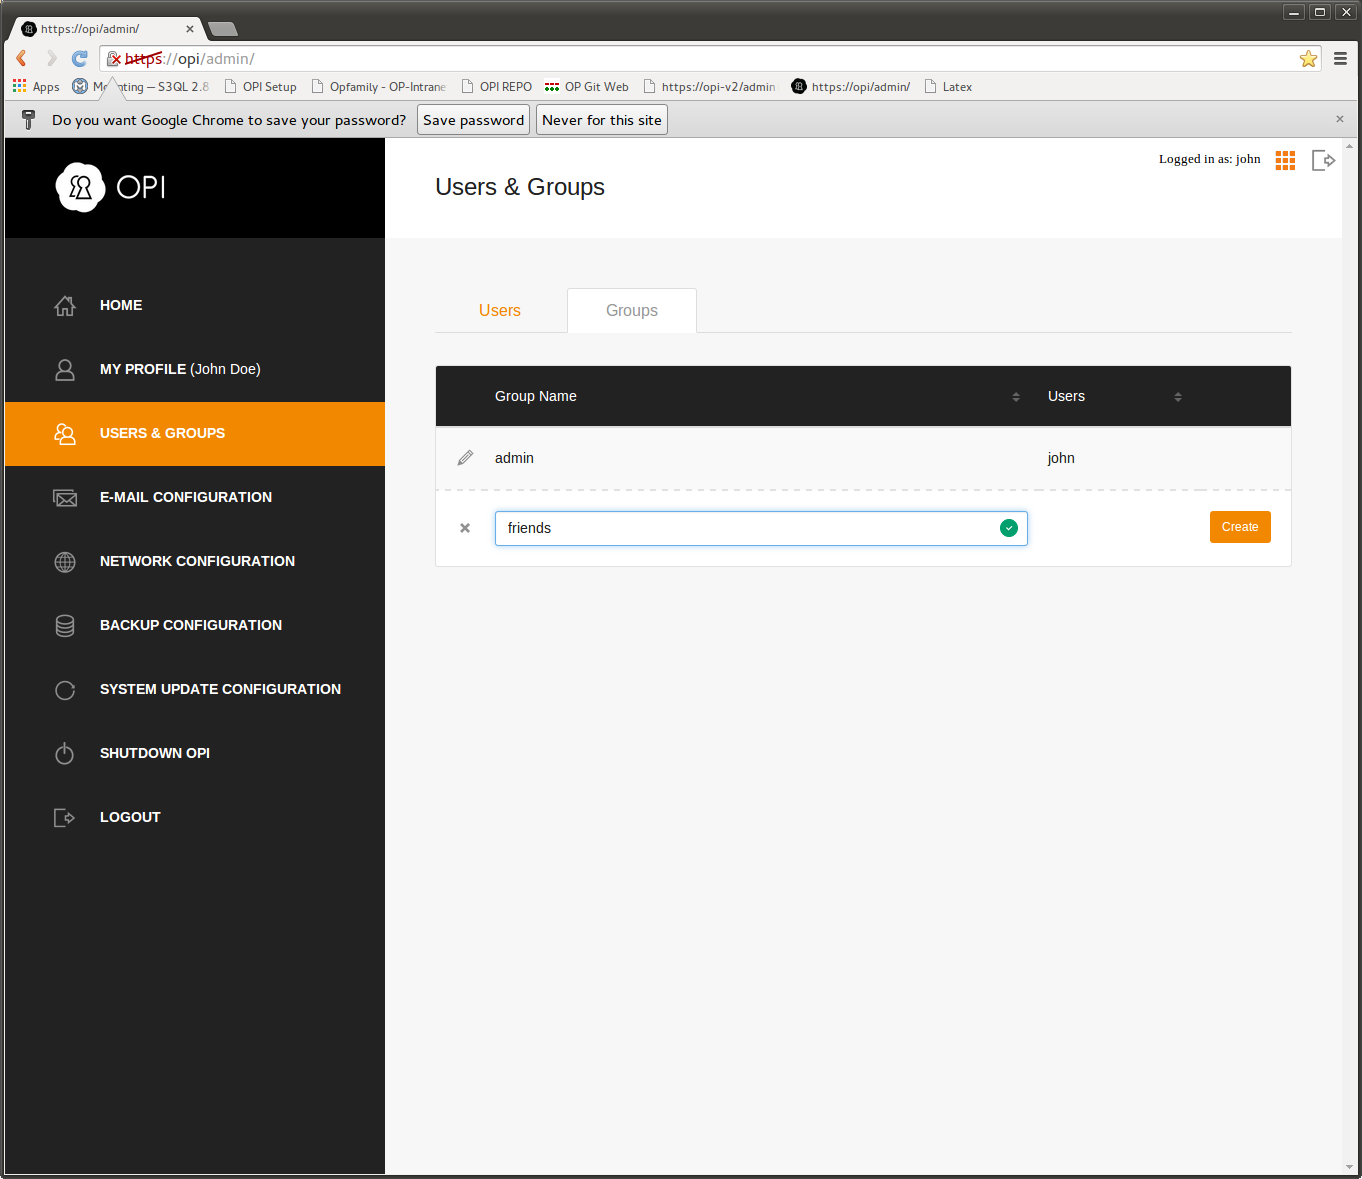
\includegraphics[width=4.93cm]{./img/groups-1}
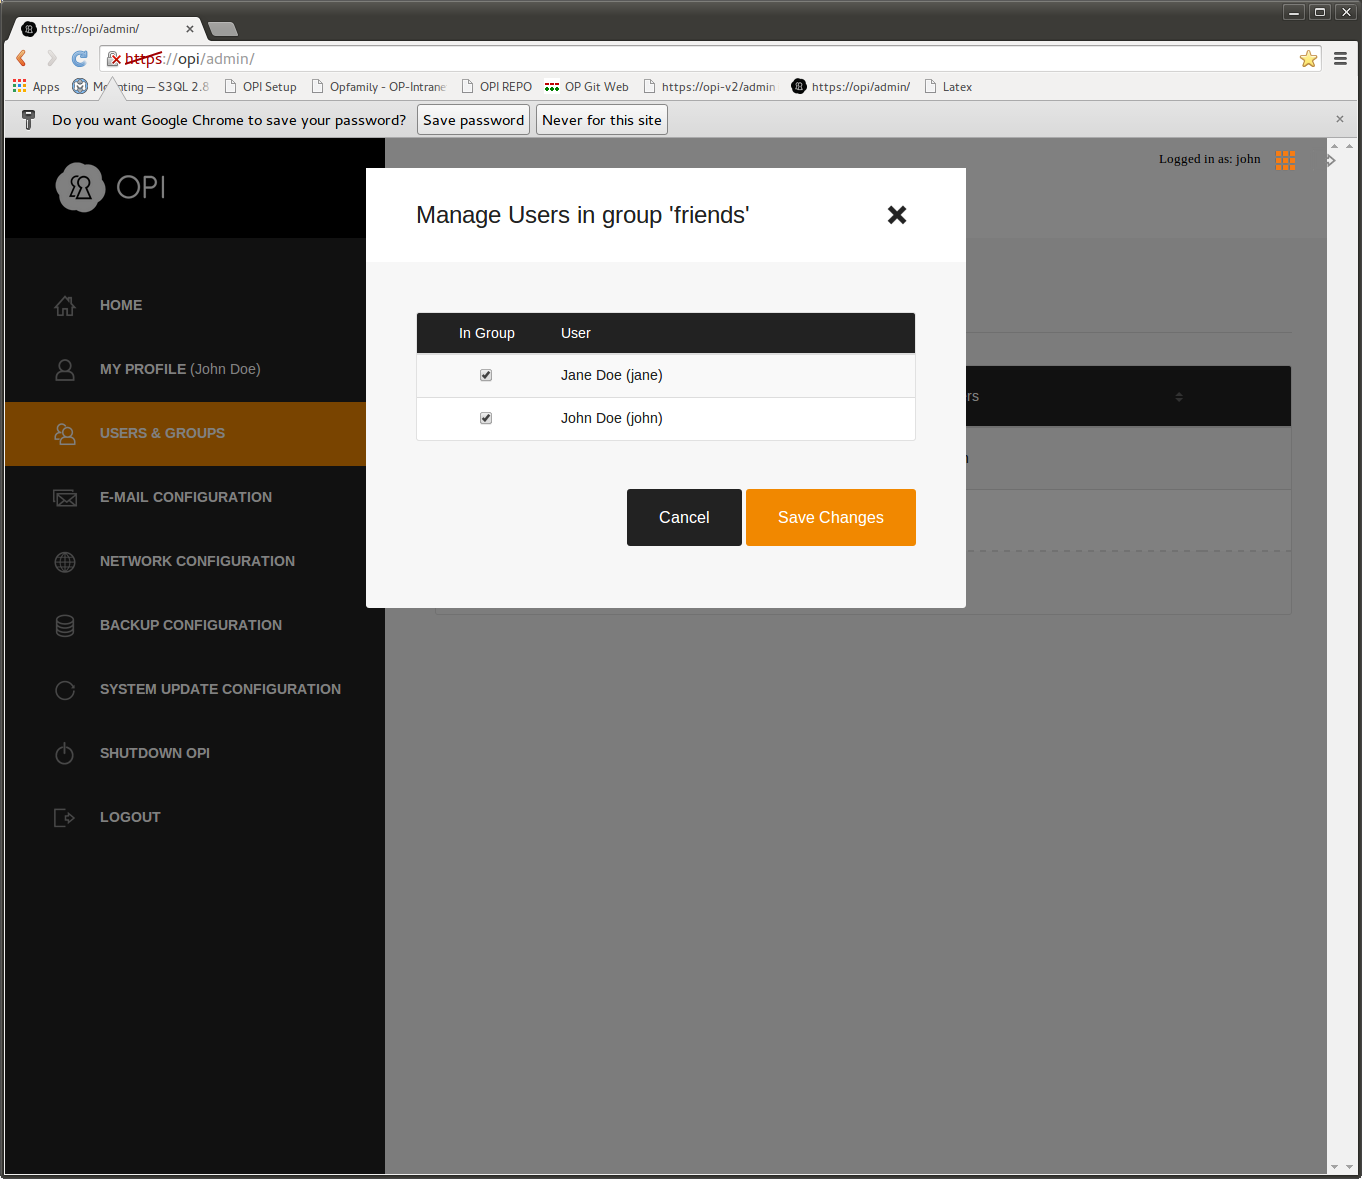
\includegraphics[width=4.93cm]{./img/groups-2}
\caption{Adding users}
\end{figure}
\newpage
\subsection{Network Configuration}
\subsubsection{Network Settings}
By default KEEP is configured to automatically retrieve an IP address from a DHCP server in the network it is connected to.
\begin{figure}[h!]
\centering
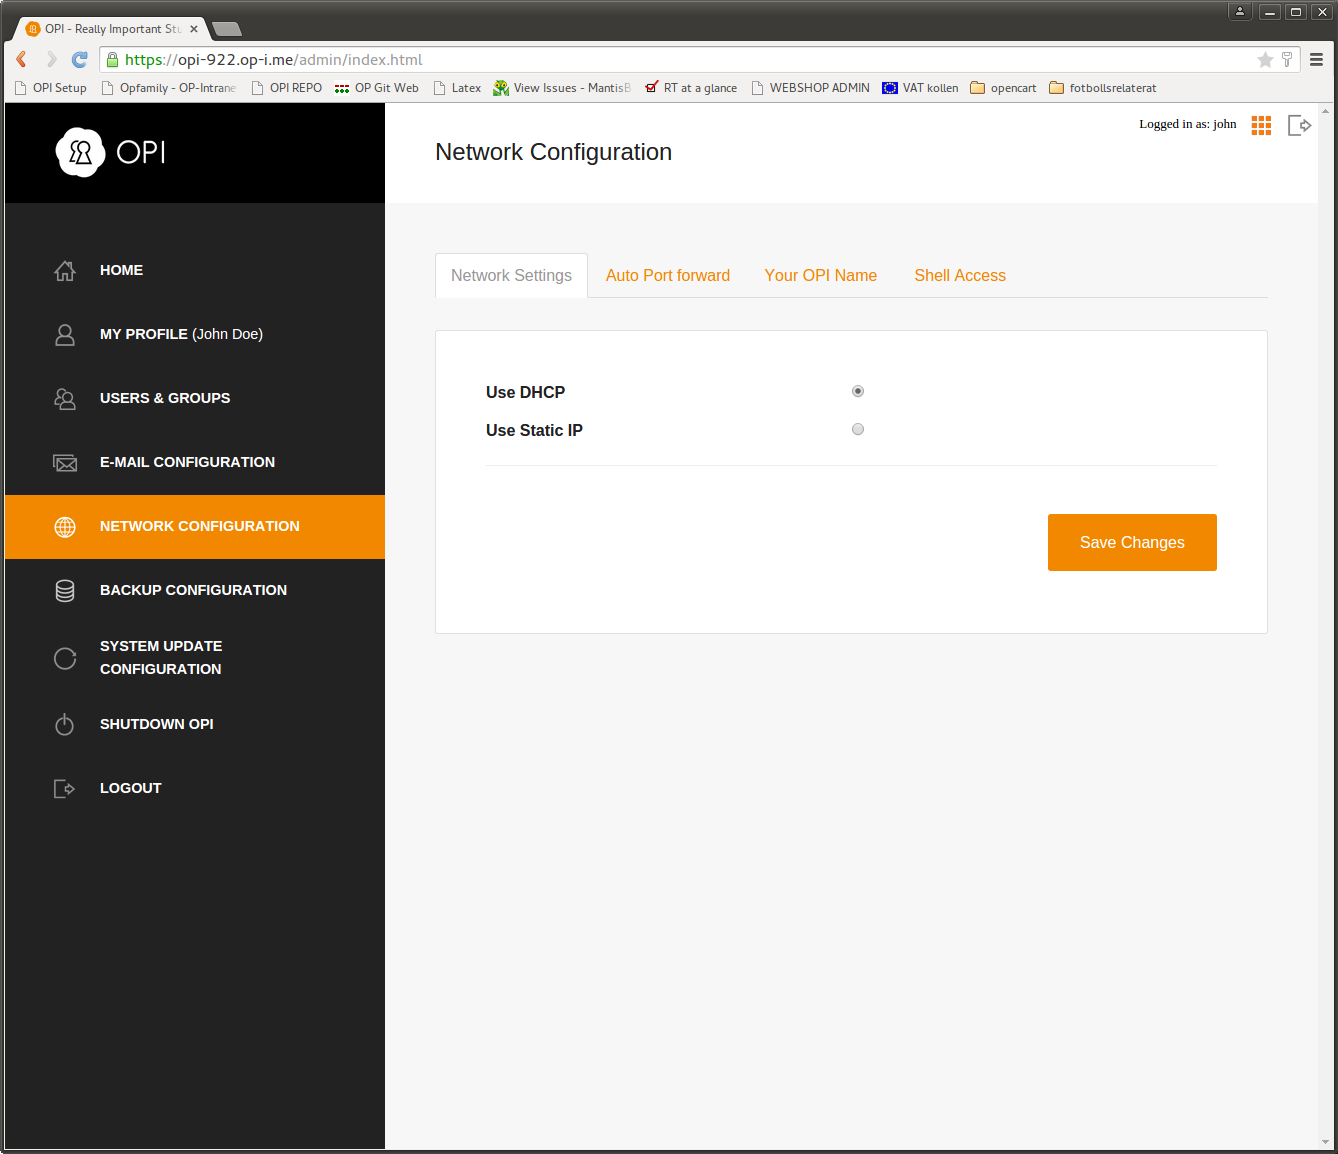
\includegraphics[width=10cm]{./img/network-config-dhcp}[h!]
\caption{Network configuration - DHCP setting}
\end{figure}
If this is not desired a static IP can be set by selecting ``Network configuration -\textgreater Network Settings''. By selecting the option "Use Static IP" a form will be presented where these settings can be entered.
\begin{figure}[h!]
\centering
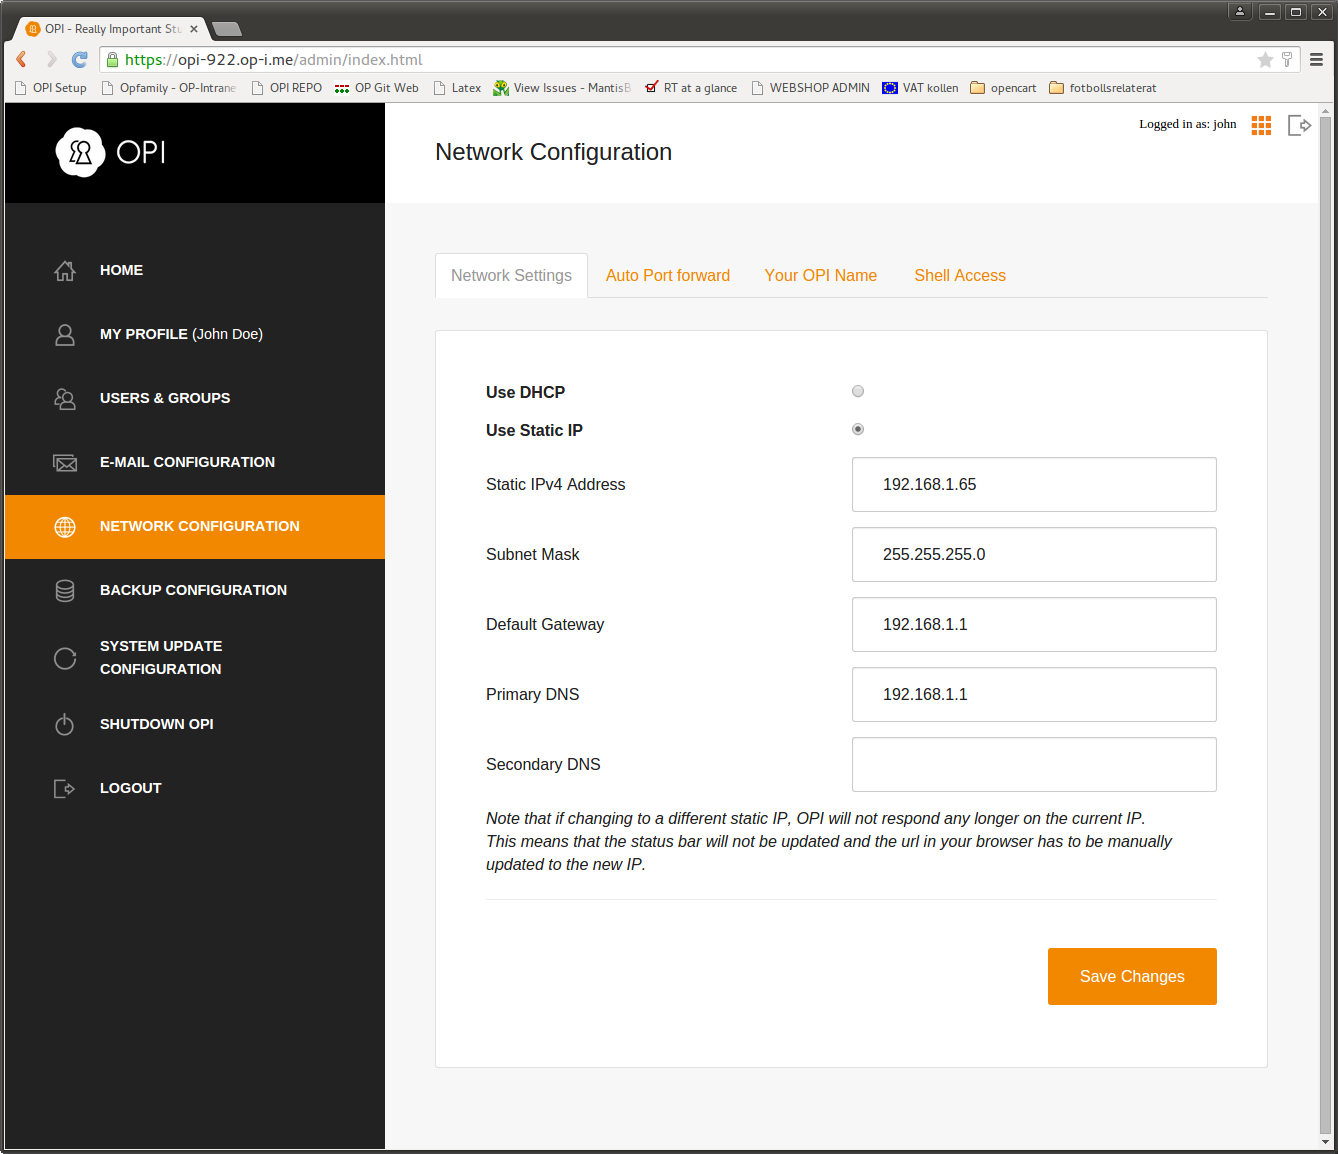
\includegraphics[width=10cm]{./img/network-config-static}
\caption{Network configuration - Static IP}
\end{figure}
\FloatBarrier
\subsubsection{Auto Port forward}
KEEP by default will try to locate an existing firewall in the network and ask that firewall to forward traffic to KEEP in order to access OPI from the Internet. This can be disabled on per port bases by clearing the check box for each port that should not be forwarded.
\begin{figure}[h!]
\centering
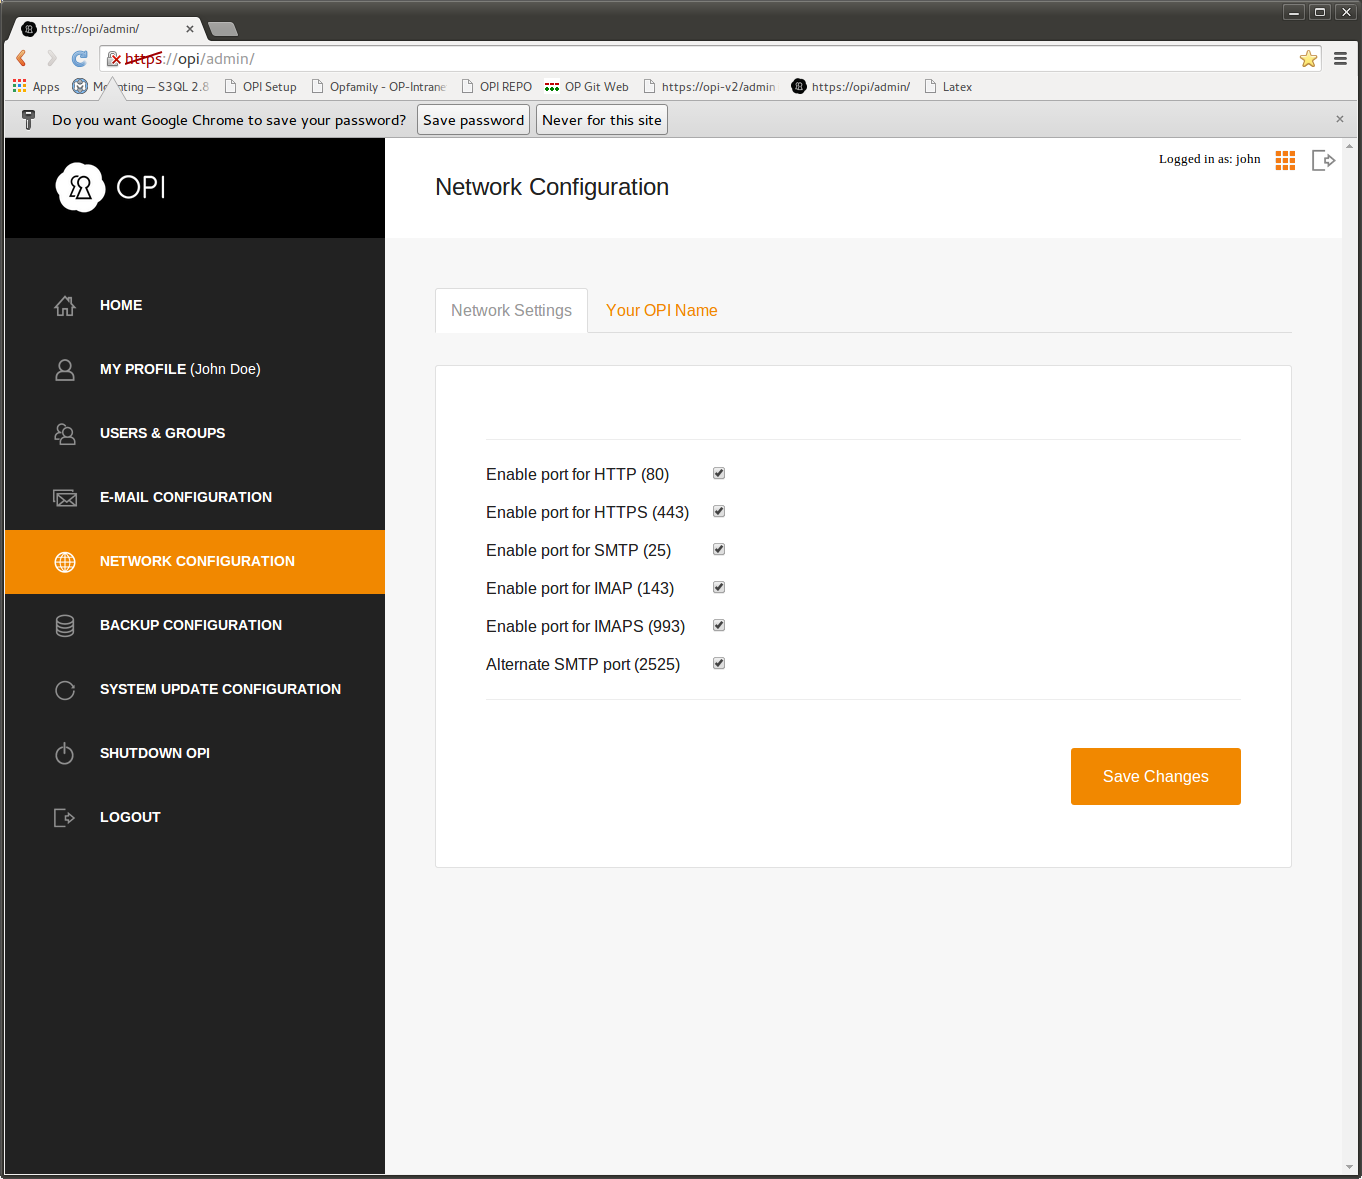
\includegraphics[width=10cm]{./img/network-config-1}
\caption{Forwarded ports}
\end{figure}
\FloatBarrier
\subsubsection{Device name}
Here the device name for the system can be changed if the one chosen during setup is not satisfactory.
If a new name is selected and the system is reachable from the internet, by default a valid certificate using \href{https://letsencrypt.org/}{Let's Encrypt} will be generated. If not a certificate signed by OpenProducts will be installed.

It is also possible to use a custom certificate by checking ``Use Custom Certificate'' and provide the key and the certificate in the text areas.
\begin{figure}[h!]
\centering
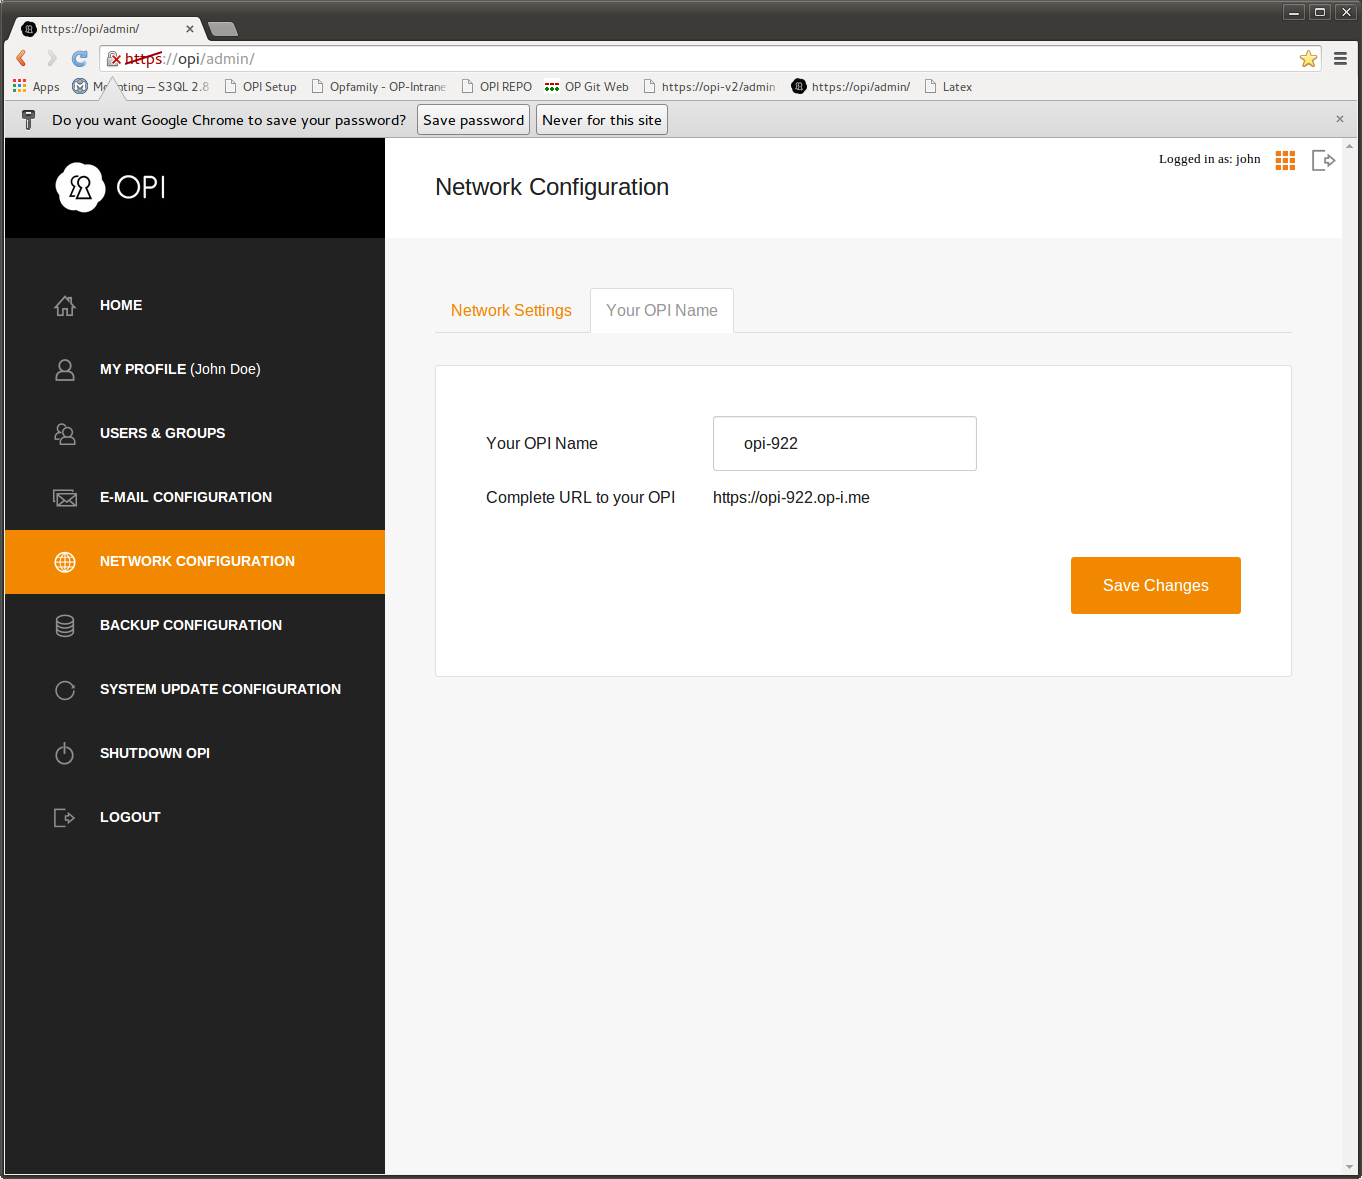
\includegraphics[width=10cm]{./img/network-opiname}
\caption{Device name}
\end{figure}
\FloatBarrier
\subsubsection{Shell access}
KEEP is an open source unit and as such we believe that it should be open in all senses. It is therefore possible to turn on shell access to KEEP by checking the "Allow shell (SSH) access to your devcie" under ``Network configuration -\textgreater Shell Access''. This will start the SSH daemon and set a password (run-time generated) for the root user. The password will be sent by email to the users in the ``admin'' group on KEEP.
\begin{figure}[h!]
\centering
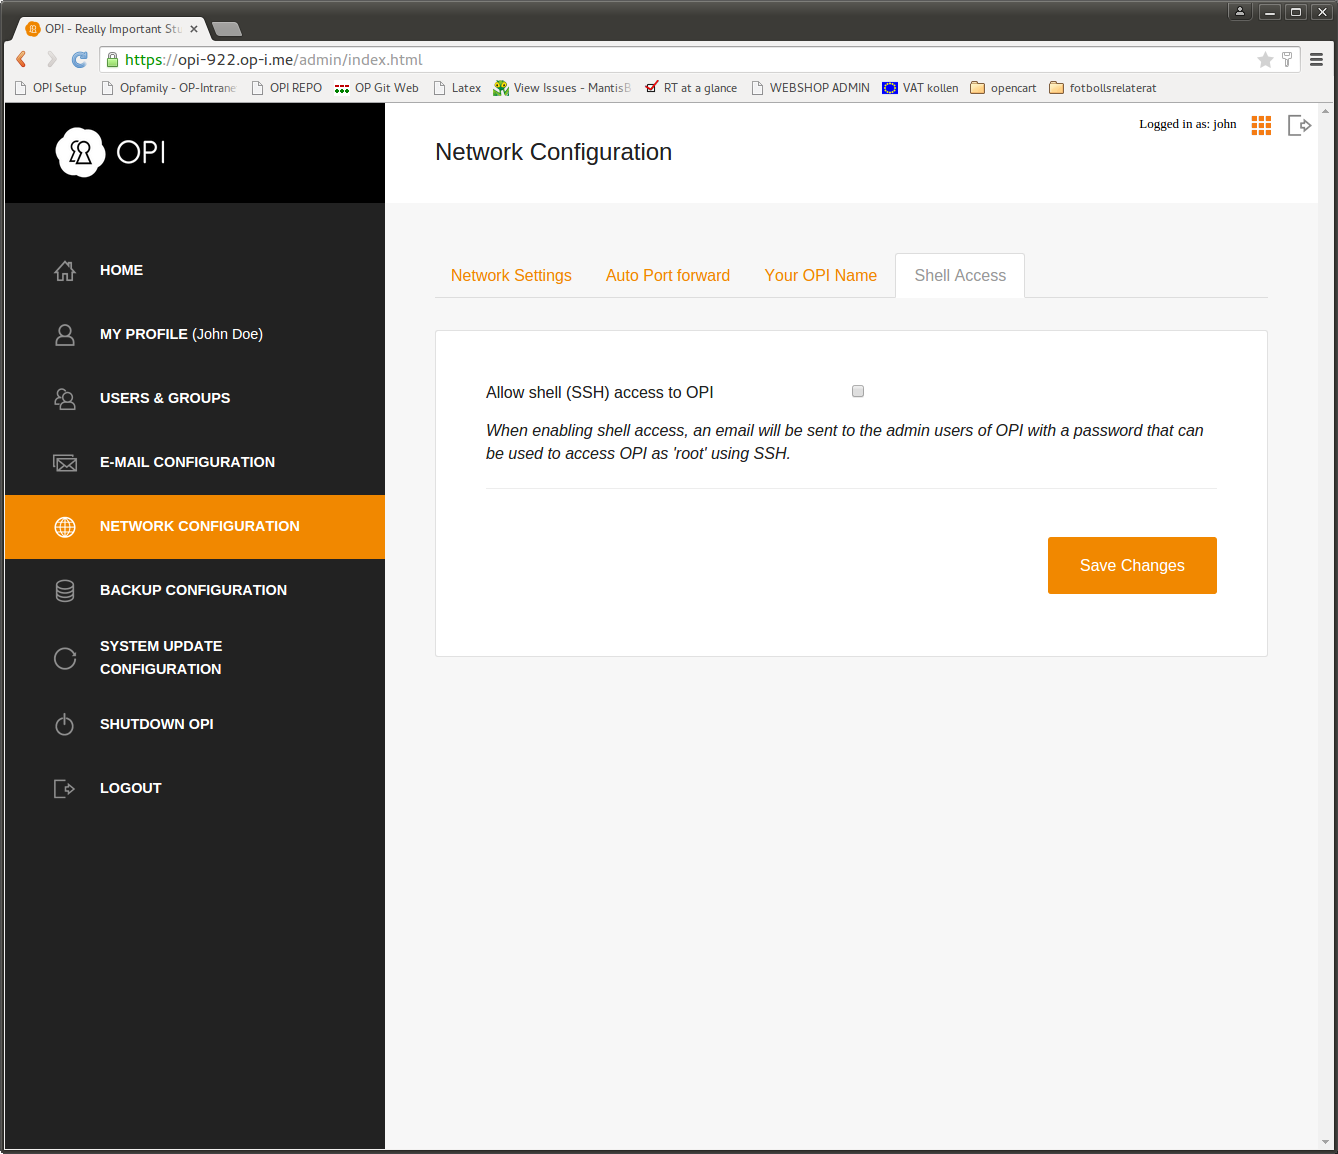
\includegraphics[width=10cm]{./img/network-shell}
\caption{Shell access}
\end{figure}
\FloatBarrier
With the username ``root'' and the generated password it is possible to log in to KEEP using SSH to gain root privileges on the system. Please use this with care, as modifications to the system might prevent built-in functions, specifically with automated updates.

\newpage
\section{Install Android Sync Applications}
To get the most out of your new system, for Android based devices we recommend that you install some application on your device.
We recommend:
\begin{itemize}
\item Mail: K9\\ \href{https://play.google.com/store/apps/details?id=com.fsck.k9}{K9 Mail}
\item Files: NextCloud\\ \href{https://play.google.com/store/apps/details?id=com.nextcloud.client}{NextCloud}
Note that the base URL to be used is https://'devicename'.mykeep.net/nc (not /owncloud)
\item Calendar and contact sync: Open Sync \\ \href{https://play.google.com/store/apps/details?id=com.deependhulla.opensync}{Open Sync}
\end{itemize}

\newpage
\section{Configure Web Mail Client}
The system automatically picks up the information of the current user and makes that available as an identity from which it is possible to send mail. There is one identity associated with each mail account configured for that user.
\begin{figure}[h!]
\centering
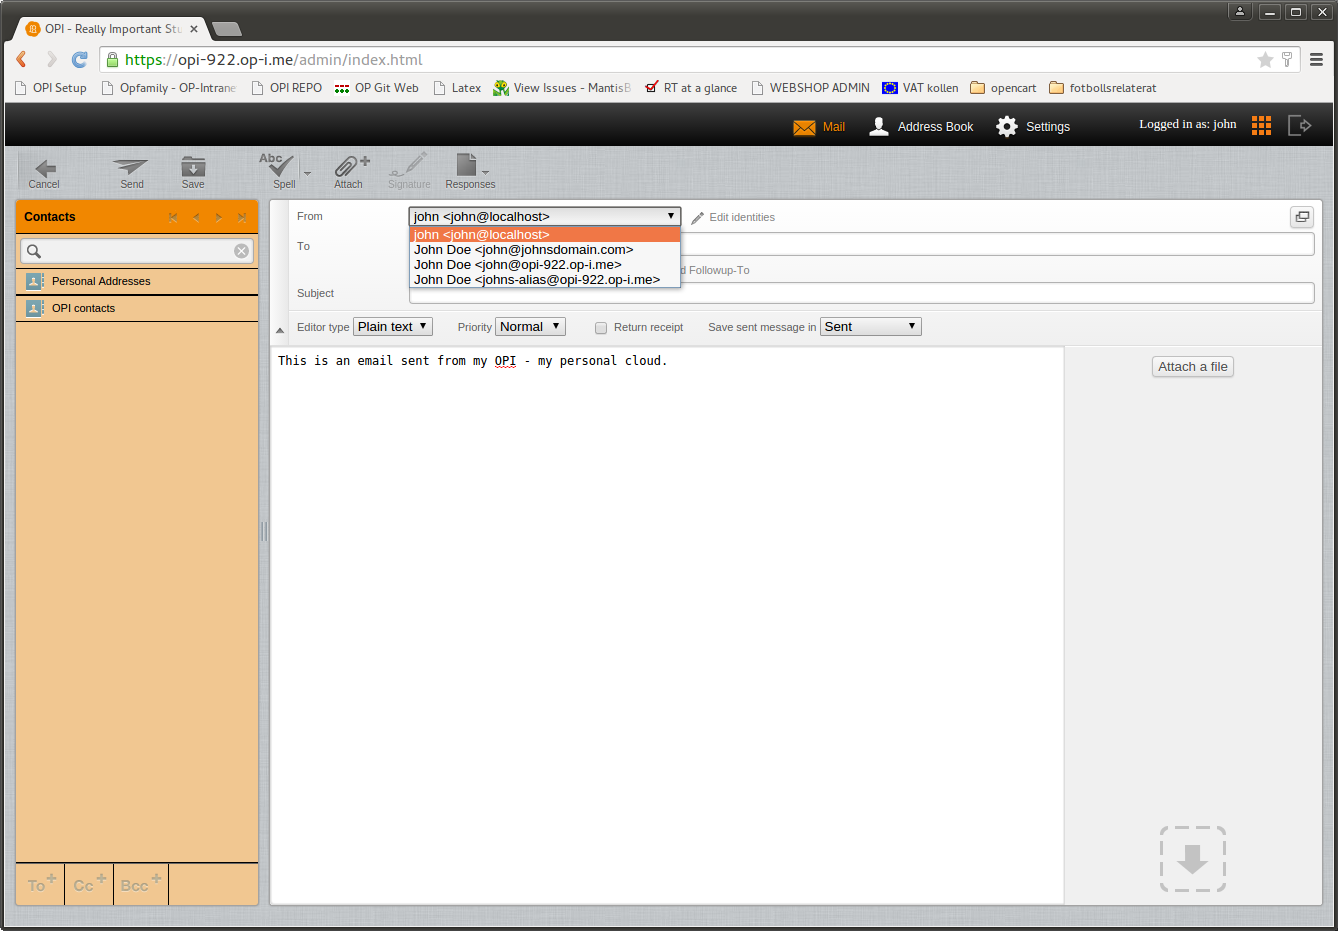
\includegraphics[width=10cm]{./img/webmail-send-identities}
\caption{Web mail sender identities}
\end{figure}
\FloatBarrier

If this is not the desired information, new identities can be added in the ``Settings'' section of the Web Mail Client.
Log in to KEEP, then using the drop down menu select the ``Mail'' application.
\begin{figure}[h!]
\centering
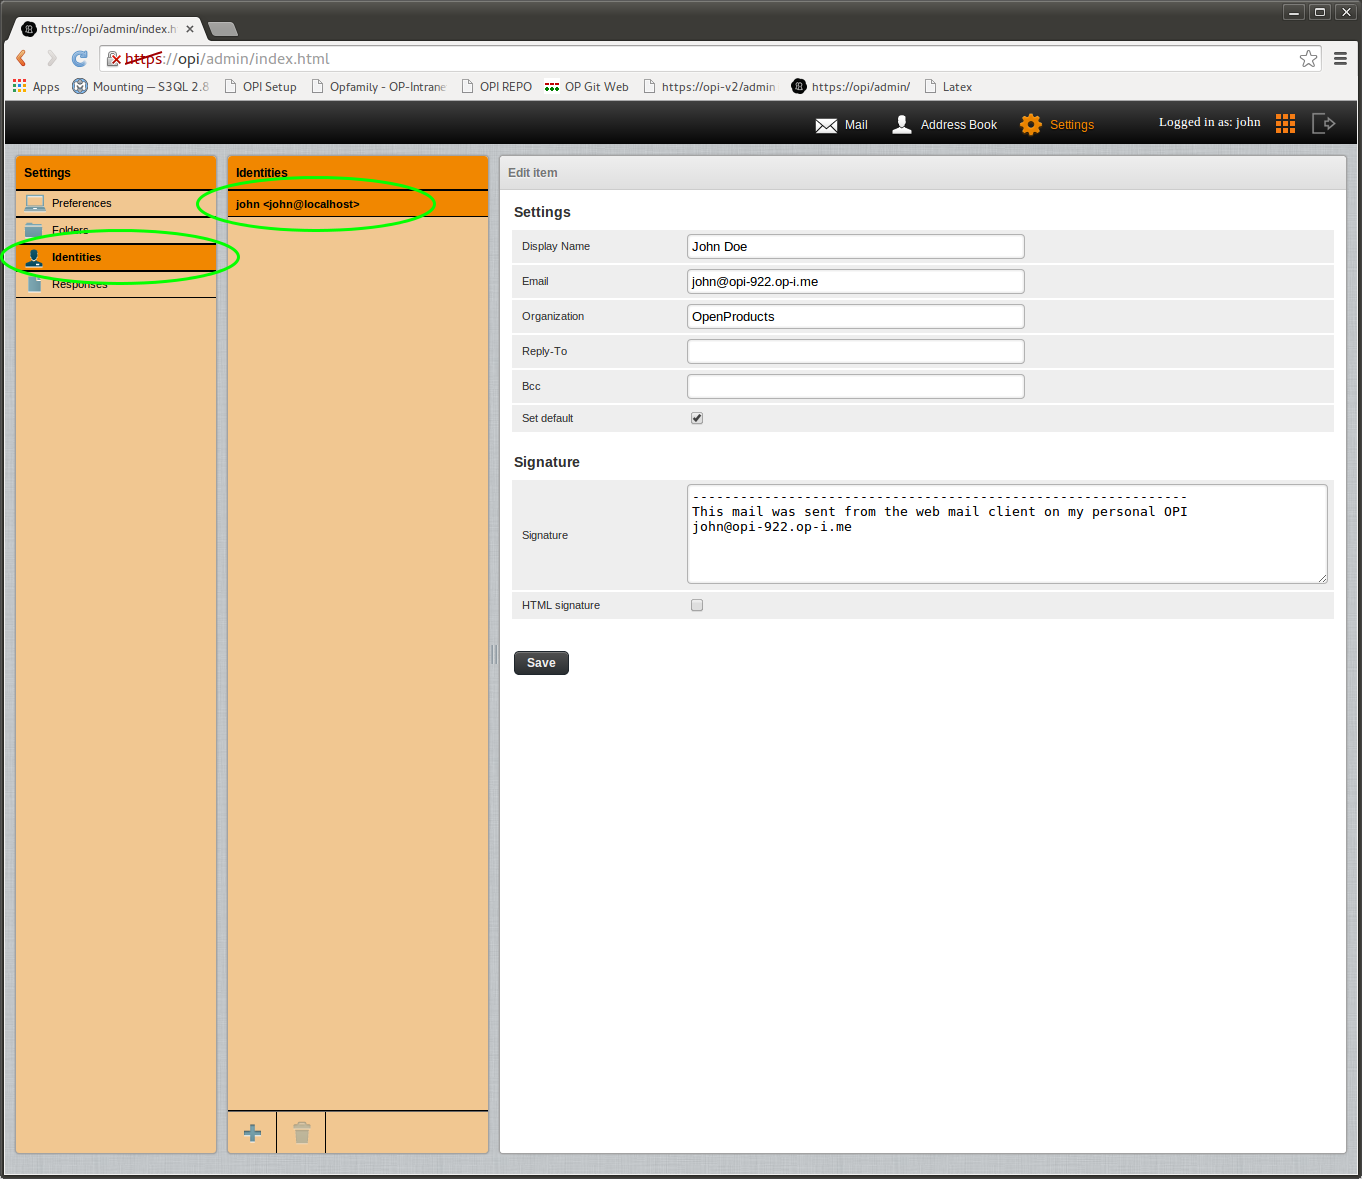
\includegraphics[width=10cm]{./img/webmail-config}
\caption{Web mail personal information}
\end{figure}
In the top right corner, select ``Settings'', then select ``Identities''.
Click that name in the center column and enter relevant information to be used as sender.
Enter the name that shall be displayed as the senders name and the email address that shall be used as the senders email.
Optionally, also a signature that will be appended to all emails sent from the web mail client can be specified.

Please note that the identities that are created by adding users and mailaccounts can not be edited here. Identities created hera are only added as information to emails sent. If an identity created here is associated with a non-exiting email account, any mail sent to that address will bounce.

\newpage
\section{Using External Clients}
\subsection{Email Settings}
The following settings should be used in order to use email with an external client, such as Mozilla Thunderbird or Evolution

\subsubsection{Incoming Mail Server}
\begin{itemize}
\item Server Type: IMAP
\item Servername: 'devicename'.mykeep.net
\item Port: 143
\item Connection Security: STARTTLS
\item Username: Your username on KEEP, (ie 'mailuser')
\item Authentication method: 'Normal password'
\end{itemize}

\subsubsection{Outgoing Mail Server (SMTP)}
\begin{itemize}
\item Server Type: SMTP
\item Servername: 'devicename'.mykeep.net
\item Port: 587
\item Connection Security: STARTTLS
\item Username: Your username on KEEP, (ie 'mailuser')
\item Authentication method: 'Normal password'
\end{itemize}

\newpage
\subsubsection{Example Using Thunderbird}
\begin{figure}[h!]
\centering
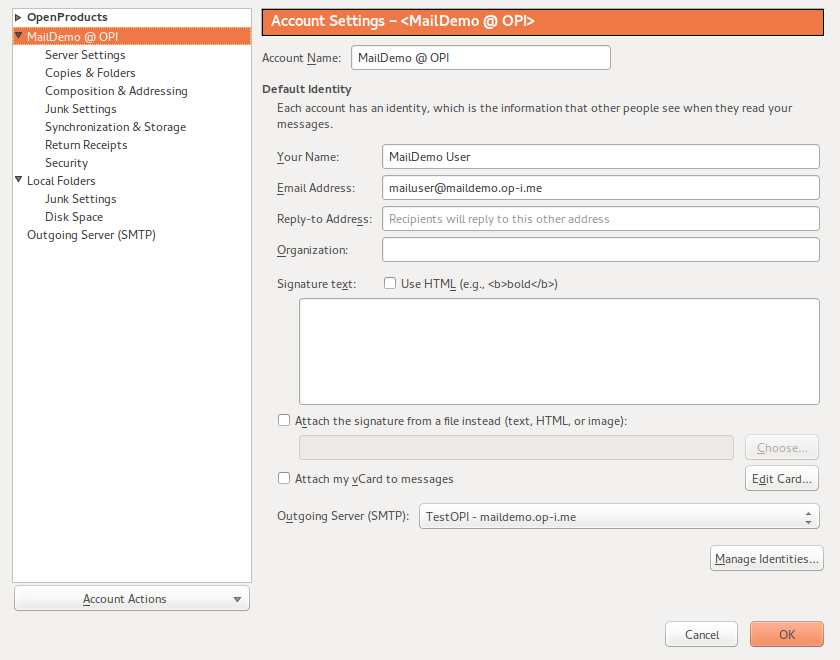
\includegraphics[width=10cm]{./img/External-clients-thunderbird1.png}
\caption{Incoming Mail Server settings}
\end{figure}
\begin{figure}[h!]
\centering
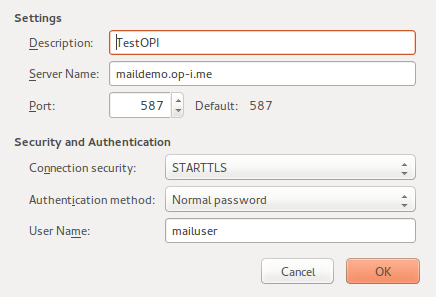
\includegraphics[width=10cm]{./img/External-clients-thunderbird2.png}
\caption{Outgoing Mail Server settings}
\end{figure}

\newpage
\subsection{Calendar settings}
Calendars on KEEP can be accessed from external applications using a standardized protocol named CalDav.

The URL's to the calendars can be found in the calendar section of the web application, see figure. First click the gear icon, then the little 'earth' symbol to display URL for the chosen calendar (see figure). Copy the URL as it will be needed below.
\begin{figure}[h!]
\centering
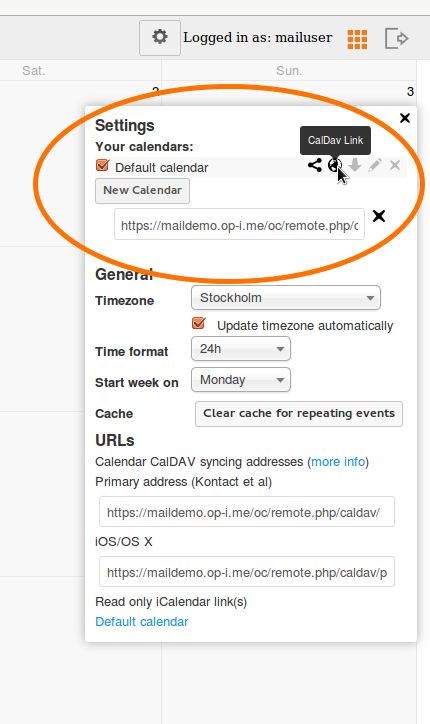
\includegraphics[width=8cm]{./img/External-clients-calendar1.png}
\caption{Calendar URL's and settings}
\end{figure}
\subsubsection{Example Using Thunderbird and Lightning}
Go to the calendar view and right click in the calendar section then click "New Calendar..." Then select that the calendar is on the network and of type "CalDav", enter the URL found above in the "Location" field.
\begin{figure}[h!]
\centering
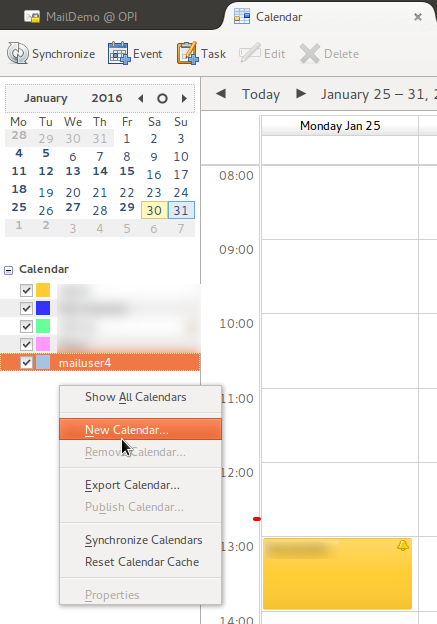
\includegraphics[width=8cm]{./img/External-clients-lightning0.png}
\caption{Adding new calendar}
\end{figure}
\begin{figure}[h!]
\centering
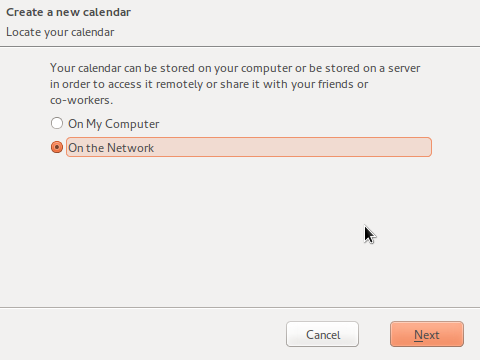
\includegraphics[width=8cm]{./img/External-clients-lightning1.png}
\caption{Select "On the Network"}
\end{figure}
\begin{figure}[h!]
\centering
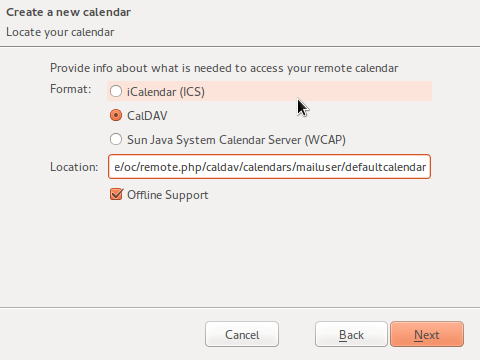
\includegraphics[width=8cm]{./img/External-clients-lightning2.png}
\caption{Select "CalDAV" and enter/paste the location found in the above step}
\end{figure}
\begin{figure}[h!]
\centering
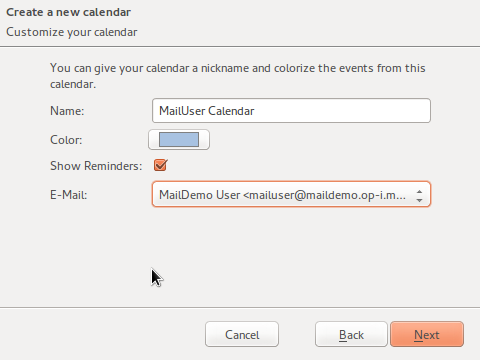
\includegraphics[width=8cm]{./img/External-clients-lightning3.png}
\caption{Give the calendar a name (can be anything) and select which email account should be associated by default with the calendar}
\end{figure}
\FloatBarrier
You might then be prompted with a security warning (depending on wether the Let's Encrypt certificate was able to be installed or not) due to that polices with self signed certificates. Accept this warning and create an exception. You will also be prompted for username and password, this is your normal KEEP username/password combination.

\newpage
\section{Further Reading}
For additional information and reading, please visit our community site where our blog and forums can be found:

\href{http://community.openproducts.com}{http://community.openproducts.com}
\newpage
\section{Contributers}
The following people have been contributing to this document:
\begin{description}
\item PA Nilsson, OpenProducts \href{http://www.openproducts.com}{http://www.openproducts.com}
\item Tor Krill, OpenProducts \href{http://www.openproducts.com}{http://www.openproducts.com}
\end{description}
Last update, \today
\end{document}
